% covtl-pipeline --- User Manual
% SPDX-License-Identifier: GPL-3.0-or-later
% Copyright (C) 2026 Frédéric Berthommier

\documentclass[11pt,a4paper]{article}

% --- Packages ---
\usepackage{lmodern}
\usepackage{graphicx}
\usepackage{xcolor}
\usepackage{geometry}
\usepackage{amsmath}
\usepackage{tcolorbox}
\tcbuselibrary{listings, breakable, skins}
\usepackage{booktabs}
\usepackage{tabularx}
\usepackage{enumitem}
\usepackage{array}
\usepackage{longtable}
\usepackage{fancyhdr}
\usepackage{titlesec}
\usepackage{listings}
\usepackage{needspace}
\usepackage{fontspec}
% The turned-h glide (U+0265) is absent from Latin Modern: borrow it
% from a system font with IPA Extensions coverage (Lucida Sans Unicode).
\newfontfamily\ipafont[Path=./, Extension=.ttf, HyphenChar=None]{.l_10646}
\newcommand{\turnh}{{\ipafont\symbol{"0265}}}
\usepackage{tikz}
\usetikzlibrary{shapes.geometric, arrows.meta, positioning, calc, fit, backgrounds}
\usepackage[
    colorlinks=true,
    linkcolor=blue!60!black,
    citecolor=blue!50!black,
    urlcolor=blue!70!black,
    bookmarks=true,
    bookmarksnumbered=true,
    unicode=true,
    pdftitle={covtl-pipeline User Manual},
    pdfauthor={Frederic Berthommier},
    pdfsubject={Articulatory text-to-speech synthesis with the Berthommier COVTL model},
    pdfkeywords={articulatory synthesis, coarticulation, polar coordinates, VocalTractLab, COVTL, speech synthesis, multi-speaker registry, language pack, expressive prosody, polar video}
]{hyperref}

% --- Geometry ---
\geometry{a4paper, top=2.5cm, bottom=2.5cm, left=2.5cm, right=2.5cm}
\setlength{\headheight}{14pt}

% --- Page style ---
\pagestyle{fancy}
\fancyhf{}
\fancyhead[L]{\small\itshape covtl-pipeline User Manual}
\fancyhead[R]{\small v1.1.0}
\fancyfoot[C]{\thepage}
\renewcommand{\headrulewidth}{0.3pt}
\renewcommand{\footrulewidth}{0pt}

% --- Section formatting ---
\titleformat{\section}{\Large\bfseries\color{blue!50!black}}{\thesection}{0.6em}{}
\titleformat{\subsection}{\large\bfseries\color{blue!40!black}}{\thesubsection}{0.5em}{}
\titleformat{\subsubsection}{\normalsize\bfseries}{\thesubsubsection}{0.4em}{}

% --- Listings (code blocks) ---
\definecolor{codebg}{HTML}{F5F5F5}
\definecolor{codeframe}{HTML}{CCCCCC}
\definecolor{codecomment}{HTML}{6A737D}
\definecolor{codekeyword}{HTML}{D73A49}
\definecolor{codestring}{HTML}{032F62}
\lstdefinestyle{shell}{
    backgroundcolor=\color{codebg},
    frame=single,
    rulecolor=\color{codeframe},
    basicstyle=\ttfamily\footnotesize,
    commentstyle=\color{codecomment}\itshape,
    keywordstyle=\color{codekeyword}\bfseries,
    stringstyle=\color{codestring},
    showstringspaces=false,
    breaklines=true,
    breakatwhitespace=true,
    numbers=none,
    xleftmargin=4pt,
    xrightmargin=4pt,
    framexleftmargin=4pt,
    framexrightmargin=4pt,
    language=bash,
    morekeywords={vtl-synth, run, text-to-wav, tract-to-mp4, inspect, plot-tract, pip, git, ffmpeg, python}
}
\lstdefinestyle{python}{
    backgroundcolor=\color{codebg},
    frame=single,
    rulecolor=\color{codeframe},
    basicstyle=\ttfamily\footnotesize,
    commentstyle=\color{codecomment}\itshape,
    keywordstyle=\color{codekeyword}\bfseries,
    stringstyle=\color{codestring},
    showstringspaces=false,
    breaklines=true,
    breakatwhitespace=true,
    numbers=none,
    xleftmargin=4pt,
    xrightmargin=4pt,
    framexleftmargin=4pt,
    framexrightmargin=4pt,
    language=Python
}
\lstdefinestyle{verbatim}{
    backgroundcolor=\color{codebg},
    frame=single,
    rulecolor=\color{codeframe},
    basicstyle=\ttfamily\footnotesize,
    showstringspaces=false,
    breaklines=true,
    breakatwhitespace=true,
    numbers=none,
    xleftmargin=4pt,
    xrightmargin=4pt,
    framexleftmargin=4pt,
    framexrightmargin=4pt
}

% --- tcolorbox callouts ---
\newtcolorbox{callout}[1][]{
    colback=blue!5,
    colframe=blue!50!black,
    fonttitle=\bfseries,
    title=#1,
    breakable=true
}
\newtcolorbox{warning}[1][]{
    colback=orange!10,
    colframe=orange!70!black,
    fonttitle=\bfseries,
    title=#1,
    breakable=true
}

% --- Orphan/widow control ---
\widowpenalty=10000
\clubpenalty=10000
\emergencystretch=1.5em
\tolerance=2000

% Long code identifiers must not run into the margin.
% (breakable-underscore experiment removed: broke math mode)

% Section headings never start in the bottom quarter of a page.
\newcommand{\sectionbreak}{\needspace{0.3\textheight}}

% --- Title ---
\title{\vspace{-1cm}\Huge\bfseries\color{blue!50!black} covtl-pipeline\\[0.3em]
\Large\mdseries\color{black!70} User Manual}
\author{\large Frédéric Berthommier\\[0.3em]
\small\texttt{fberthommier@users.noreply.github.com}}
\date{\small Version 1.1.0 --- September 2026\\[0.2em]
\textit{Licensed under GPL-3.0-or-later}}

\begin{document}
\maketitle
\thispagestyle{empty}
\vspace{0.2em}
\begin{abstract}
\noindent
\textbf{covtl-pipeline} is a Python package and command-line tool
(\texttt{vtl-synth}) that converts raw English text --- or direct SAMPA
phonetic input --- into an articulatory speech signal and an animated video
of the vocal-tract sagittal cross-section. Its synthesis engine implements
the \textbf{Berthommier COVTL articulatory model}: every phoneme carries a
target defined by \emph{polar coordinates} \((\rho,\theta)\) in a compact
two-dimensional phonetic plane, and coarticulation emerges from the
\emph{superposition} of a continuous vocalic trajectory with transient
consonantal gestures projected onto disjoint sets of VocalTractLab
parameters. A tag-based extension engine drives voicing, nasality,
laterality, glottal effort and F0, and a syllabic trajectory engine
(\emph{syltraj}) shapes the consonant/vowel arcs, inter-word pauses and
phrase-final holds. The 400\,Hz tract sequence is synthesized
\emph{directly} by this model --- there is no intermediate gestural-score
stage --- and audio is rendered by \textbf{VocalTractLab~2.4}
(Peter Birkholz, TU~Dresden) through the
\texttt{vocaltractlab-cython} wheel with the active registry speaker
(default: JD3). This manual
documents the model in detail (polar targets, projection coefficients,
coarticulation rules), the command-line interface, the Python API, the
file formats, and the underlying mechanisms and constants. Version
1.1.0 ships the package as an integrated pack: a five-speaker
registry with a one-command reversible selector
(\texttt{install\_speaker.py}), a six-language pack
(\texttt{setup\_lang.py}), an expressive-prosody option
(\texttt{-{}-expressive}) and a dual-panel polar video
(\texttt{-{}-polar}); each add-on has its own companion manual in
\texttt{docs/} (\S\ref{subsec:docmap}).
\end{abstract}

\vfill
\begin{callout}[At a glance]
\begin{itemize}[leftmargin=1.5em,itemsep=2pt]
\item \textbf{Pipeline:} text \(\to\) SAMPA \(\to\) polar targets
      \((\rho,\theta)\) \(\to\) 100\,Hz model trajectory \(\to\)
      \texttt{.tract} (400\,Hz, 19 + 11 params) \(\to\) \texttt{.wav}
      (44.1\,kHz) \(\to\) \texttt{.mp4}
\item \textbf{CLI:} \texttt{vtl-synth run "this is easy for us" -o ./out}
\item \textbf{Python API:} \texttt{from vtl\_synth import Pipeline}
\item \textbf{Model:} Berthommier COVTL --- polar phonetic targets,
      selector-based coarticulation, S-curve arcs
\item \textbf{Synthesizer:} VocalTractLab 2.4 via
      \texttt{vocaltractlab-cython}
\item \textbf{Speakers:} five-speaker registry (jd3, s1, s2, m01,
      w02) with a one-command reversible selector
\item \textbf{Languages:} six-language pack en/fr/es/de/it/pt with
      calibrated vowel targets (default: en)
\item \textbf{Options:} expressive prosody (\texttt{-{}-expressive})
      and dual-panel polar video (\texttt{-{}-polar})
\item \textbf{License:} GPL-3.0-or-later (inherited from upstream VTL
      components)
\end{itemize}
\end{callout}

\newpage
\tableofcontents
\newpage

%==============================================================================
\section{Introduction}\label{sec:intro}
%==============================================================================

\textbf{covtl-pipeline} is an articulatory text-to-speech and
video-synthesis pipeline. Given raw English text, it produces:

\begin{itemize}[leftmargin=1.5em]
\item a phonemic transcription in the engine SAMPA notation,
\item a tract sequence (\texttt{.tract}) giving the 19 VocalTractLab tract
      parameters and 11 glottis parameters at 400\,Hz,
\item an audio waveform (\texttt{.wav}) at \(44\,100\,\mathrm{Hz}\),
      synthesized by VocalTractLab,
\item an animated MP4 showing the sagittal cross-section of the vocal
      tract synchronized with the waveform.
\end{itemize}

The synthesis engine is the \textbf{Berthommier COVTL articulatory model},
a compact mathematical model of speech production in which phonetic
knowledge is encoded geometrically:

\begin{itemize}[leftmargin=1.5em]
\item every phoneme --- vowel or consonant --- is a point
      \(z = \rho\,e^{i\theta}\) in a \emph{polar phonetic plane}; the
      radius \(\rho\) is an aperture/closure magnitude and the angle
      \(\theta\) is the direction of the articulatory gesture;
\item the plane is projected linearly onto the 15 controlled parameters of
      a Maeda-type vocal-tract model, so that a single \((\rho,\theta)\)
      target simultaneously coordinates jaw, lips, hyoid, tongue body,
      tongue tip, tongue base and tongue sides;
\item coarticulation is not a post-hoc smoothing: it is the structural
      \emph{superposition} of a continuous \emph{vocalic branch} and
      transient \emph{consonantal branch}, each projected onto its own
      subset of parameters (its \emph{selector}). During a labial stop the
      tongue keeps following the vowel; during a lingual consonant the jaw
      and lips keep following it;
\item source characteristics (voicing, nasality, laterality, glottal
      effort, F0) are driven by a tag-based extension engine whose events
      are \emph{indexed by the articulatory trajectory itself} --- the
      source inherits the coarticulation of the tract.
\end{itemize}

The model is coupled to \textbf{VocalTractLab 2.4} (VTL), the
physiological articulatory synthesizer developed by Peter Birkholz and
collaborators at TU Dresden. VTL converts each 400\,Hz vocal-tract state
into cross-sectional areas and runs its aerodynamic-acoustic simulation to
produce the 44.1\,kHz waveform. The package depends on the
\texttt{vocaltractlab-cython} wheel (Paul Krug's Cython binding of VTL),
which also provides the SVG export of vocal-tract shapes used by the video
pipeline. The repository and packaging layout follow the
\href{https://github.com/FBerthommier/vtl-pipeline}{vtl-pipeline}
reference repository; the synthesis path itself is entirely different
(see \S\ref{sec:differences}).

\subsection*{Key features}

\begin{itemize}[leftmargin=1.5em]
\item End-to-end pipeline from raw text to MP4 in a single command, or
      direct SAMPA input with \texttt{-{}-phonetic}.
\item Polar-coordinate phonetic targets with documented, calibrated
      coefficient tables (\S\ref{sec:polar}).
\item Selector-based coarticulation with lightened selectors, contextual
      consonant targets, cluster scoping and vowel-to-vowel background
      arcs (\S\ref{sec:coart}).
\item Tag-based source model: voicing, VOT by place of articulation,
      nasality with carry-over, glottal effort and F0 declination
      (\S\ref{sec:source}).
\item Syllabic trajectory engine (\texttt{syl}) with pause handling and
      phrase-final holds; a legacy superposition-graph engine remains
      selectable (\S\ref{sec:syltraj}).
\item Inspectors for the tract sequence: \texttt{inspect} (tables,
      ranges) and the graphical \texttt{plot-tract}.
\item Per-speaker non-regression baselines (jd3, s1, s2, m01, w02)
      checked by pytest; the repository ships a lightened quick suite
      (\S\ref{sec:dev}).
\item Four integrated add-ons --- multi-speaker registry, language
      pack, expressive prosody, polar video --- each documented in its
      own companion manual (\S\ref{subsec:docmap}).
\end{itemize}

\subsection{Documentation map}\label{subsec:docmap}

The \texttt{docs/} folder carries five manuals, written to be read
independently:

\begin{description}[leftmargin=2em]
\item[\texttt{manual.pdf}] this reference manual: the COVTL model,
      the CLI and Python API, the file formats.
\item[\texttt{speakers.pdf}] the multi-speaker registry: the five
      speakers and their provenance, the selector
      \texttt{install\_speaker.py}, and the two adaptation chains
      (DVTD construction; official-speaker patching).
\item[\texttt{language\_pack.pdf}] the language pack: six languages,
      installation, switching, calibration and verification through
      \texttt{setup\_lang.py}.
\item[\texttt{expressive\_prosody.pdf}] the expressive-prosody
      option: syntactic breathing and sculpted F0 contour.
\item[\texttt{polar\_visualization.pdf}] the dynamic polar video:
      two-branch display of the articulation, \texttt{.polar}
      format, dual-panel MP4.
\end{description}

%==============================================================================
\section{Quick start}\label{sec:quickstart}
%==============================================================================

\subsection{Prerequisites}

\begin{itemize}[leftmargin=1.5em]
\item Python 3.9 or newer.
\item No system \texttt{ffmpeg} is required: the \texttt{imageio-ffmpeg}
      wheel bundles a private ffmpeg binary for MP4 encoding.
\item About 200\,MB of disk for the Python packages.
\end{itemize}

\subsection{Installation}

\begin{lstlisting}[style=shell]
git clone https://github.com/fberthommier/covtl-pipeline.git
cd covtl-pipeline
pip install .            # or: pip install -e .   (development)

# Optional: PNG figures of .tract files (plot-tract)
pip install ".[plot]"    # pulls matplotlib

# Verify
vtl-synth --help
\end{lstlisting}

The install pulls \texttt{numpy}, \texttt{scipy},
\texttt{vocaltractlab-cython}, \texttt{Pillow}, \texttt{imageio-ffmpeg}
and \texttt{cmudict} automatically. The console script
\texttt{vtl-synth} lands in the Python \emph{Scripts} folder; with
\texttt{pip install -{}-user} on Windows this is
\texttt{\%APPDATA\%\textbackslash Python\textbackslash Python39\textbackslash Scripts}
--- add it to \texttt{PATH}, call it by full path, or use the provided
\texttt{launch.bat}. Under Python 3.9, if pip tries to build
\texttt{vocaltractlab-cython} from source, install
\texttt{vocaltractlab-cython==0.0.13} instead (full synthesis and video
path available; four optional analysis helpers raise a clear error).
The polar video (\texttt{-{}-polar}) and \texttt{plot-tract}
additionally require \texttt{matplotlib} (\texttt{pip install
".[plot]"}).

\subsection{First run}

The shipped tree is delivered in the reference state (speaker
\texttt{jd3}, language \texttt{en}). The \texttt{ACTIVE\_SPEAKER}
marker is not part of the package: create it once before the first
synthesis with \texttt{python install\_speaker.py list}
(\S\ref{sec:multispeaker}).

\begin{lstlisting}[style=shell]
vtl-synth run "this is easy for us" -o ./out
\end{lstlisting}

This produces the following artifacts in \texttt{./out/} (real output,
default configuration):

\begin{lstlisting}[style=verbatim]
this_is_easy_for_us.tract   268,286 bytes   952 frames x (19 tract + 11 glottis) @ 400 Hz
this_is_easy_for_us.wav     209,484 bytes   PCM 16-bit, mono, 44100 Hz, 2.37 s
this_is_easy_for_us.mp4     239,001 bytes   H.264 960x840 @ 25 fps + AAC, 2.40 s
this_is_easy_for_us.txt          20 bytes   the SAMPA transcript: Dis.iz.i.zi.fOR.@s
\end{lstlisting}

The video shows the sagittal cross-section of the vocal tract; the audio
is normalized to \(90\,\%\) of full scale by the pipeline.

\subsection{Inspecting the output}

\begin{lstlisting}[style=shell]
# Summary + per-parameter min/max/mean of a .tract
vtl-synth inspect ./out/this_is_easy_for_us.tract --states 2 --ranges

# Graphical counterpart: 400 Hz trajectory of each parameter
vtl-synth plot-tract ./out/this_is_easy_for_us.tract --which all -o ./out/tract.png
vtl-synth plot-tract ./out/this_is_easy_for_us.tract --params JX JA TTX TTY

# Re-render a video from an existing tract + wav (no re-synthesis)
vtl-synth tract-to-mp4 ./out/this_is_easy_for_us.tract ./out/this_is_easy_for_us.wav \
    -o ./out/this_is_easy_for_us_hd.mp4
\end{lstlisting}

%==============================================================================
\section{The COVTL model I: phonetic targets in polar coordinates}\label{sec:polar}
%==============================================================================

This section and the next describe the core of the synthesis engine: how
phonemes are represented, how the plane is mapped onto vocal-tract
parameters, and how coarticulation is obtained. The reference publications
are listed in \S\ref{sec:license}; the implementation lives in
\texttt{vtl\_synth/core/polar.py}, \texttt{projection.py},
\texttt{constants.py} and \texttt{syltraj.py}.

The global architecture of the model is a sum of three contributions:
\begin{equation}
\mathrm{VTL}(t) \;=\; B(t) \;+\; E_{\mathrm{source}}(t) \;+\; E_{\mathrm{ortho}}(t),
\label{eq:global}
\end{equation}
where \(B(t)\) is the \emph{Berthommier polar core}: the 15 COVTL tract
parameters trajectory built from polar targets; \(E_{\mathrm{source}}(t)\)
groups the extension parameters produced by the tag/envelope engine
(velum VS/VO and the 11 glottis parameters); and \(E_{\mathrm{ortho}}(t)\)
is the orthogonal branch (TS3 tongue-side shape and the speaker-derived
VS), read from the JD3 speaker file (\S\ref{sec:ortho}).

\subsection{The \((\rho,\theta)\) phonetic plane}\label{subsec:plane}

Every phoneme is a point
\begin{equation}
z \;=\; \rho\, e^{\,i\theta}, \qquad \rho \ge 0,\; \theta \in [0, 2\pi),
\label{eq:z}
\end{equation}
in a complex \emph{phonetic plane}:

\begin{itemize}[leftmargin=1.5em]
\item \(\rho\) is a dimensionless \textbf{aperture/closure magnitude}.
      \(\rho = 0\) is the origin (minimum displacement); \(\rho \le 1\)
      covers the vowel space; \(\rho > 1\) --- beyond the unit circle ---
      is the \emph{constriction/occlusion region} used by consonants. The
      per-parameter amplitude \(c_0\) (Table~\ref{tab:co}) carries the
      physical (centimeter) scaling.
\item \(\theta\) is the \textbf{direction of the articulatory gesture}.
      The convention is fixed by the three corner vowels of the Maeda
      reference vowel triangle:
      \(/a/ = \pi\) (\(180^\circ\), low-open-central),
      \(/i/ = 5\pi/3\) (\(300^\circ\), palatal-front),
      \(/u/ = \pi/3\) (\(60^\circ\), velar-back-round).
\end{itemize}

\begin{figure}[t]
\centering
\begin{tikzpicture}[scale=3.0, >={Stealth[length=4pt]}]
  % axes and rays
  \draw[->, black!60] (-1.75,0) -- (1.75,0);
  \draw[->, black!60] (0,-1.75) -- (0,1.75);
  \draw[black!25] (0,0) -- (60:1.62);
  \draw[black!25] (0,0) -- (300:1.62);
  \node[font=\scriptsize, black!60, below left] at (-0.02,0.02) {$0$};
  \node[font=\scriptsize, black!60] at (0,1.82) {$90^\circ$};
  \node[font=\scriptsize, black!60] at (-1.82,0) {$180^\circ$};
  \node[font=\scriptsize, black!60] at (0,-1.82) {$270^\circ$};
  \node[font=\scriptsize, black!40] at (60:1.72) {$60^\circ$};
  \node[font=\scriptsize, black!40] at (300:1.72) {$300^\circ$};
  % unit circle (vowel frontier)
  \draw[dashed, black!55] (0,0) circle (1);
  \node[font=\scriptsize, black!55] at (135:1.30) {$\rho=1$};
  % occlusion ring
  \draw[dotted, black!30] (0,0) circle (1.45);
  % neutral point
  \draw[black!60, fill=white] (180:0.42) circle (0.9pt);
  \node[font=\scriptsize, black!60, below] at (180:0.40) {rest};
  % ---------------- vowels (filled) ----------------
  \fill[blue!60!black] (180:1.000) circle (1.1pt);
  \node[font=\scriptsize\bfseries, blue!60!black, left] at (180:1.02) {a};
  \fill[blue!60!black] (300:0.600) circle (1.1pt);
  \node[font=\scriptsize\bfseries, blue!60!black, right] at (300:0.60) {i};
  \fill[blue!60!black] (60:0.550) circle (1.1pt);
  \node[font=\scriptsize\bfseries, blue!60!black, right] at (60:0.52) {u};
  \fill[blue!60!black] (262.5:0.988) circle (1.1pt);
  \node[font=\scriptsize, blue!60!black, below right] at (263:1.00) {e};
  \fill[blue!60!black] (204.1:0.594) circle (1.1pt);
  \node[font=\scriptsize, blue!60!black, left] at (204:0.59) {E};
  \fill[blue!60!black] (104.7:1.000) circle (1.1pt);
  \node[font=\scriptsize, blue!60!black, above right] at (105:1.02) {o};
  \fill[blue!60!black] (149.9:1.000) circle (1.1pt);
  \node[font=\scriptsize, blue!60!black, above] at (150:1.04) {O};
  \fill[blue!60!black] (174.9:0.894) circle (1.1pt);
  \node[font=\scriptsize, blue!60!black, above left] at (174:0.91) {6};
  \fill[blue!60!black] (177.9:0.722) circle (1.1pt);
  \node[font=\scriptsize, blue!60!black, right] at (179:0.74) {9};
  \fill[blue!60!black] (180:0.7167) circle (1.1pt);
  \node[font=\scriptsize\bfseries, blue!60!black, below, yshift=1pt] at (180:0.69) {@};
  \fill[blue!60!black] (260.6:0.519) circle (1.1pt);
  \node[font=\scriptsize, blue!60!black, left] at (260:0.53) {y};
  \fill[blue!60!black] (226.1:0.396) circle (1.1pt);
  \node[font=\scriptsize, blue!60!black, above left] at (226:0.39) {2};
  % ---------------- consonants (crosses) ----------------
  \draw[red!70!black, thick] (50:1.06) -- ++(150:0.035) (50:1.06) -- ++(-30:0.035)
      (50:1.06) -- ++(30:0.035) (50:1.06) -- ++(210:0.035);
  \node[font=\scriptsize, red!70!black, above right] at (50:1.07) {b, m};
  \draw[red!70!black, thick] (270:1.10) -- ++(0:0.035) (270:1.10) -- ++(180:0.035)
      (270:1.10) -- ++(90:0.035) (270:1.10) -- ++(270:0.035);
  \node[font=\scriptsize, red!70!black, below left] at (270:1.10) {d};
  \draw[red!70!black, thick] (60:1.45) -- ++(0:0.035) (60:1.45) -- ++(180:0.035)
      (60:1.45) -- ++(90:0.035) (60:1.45) -- ++(270:0.035);
  \node[font=\scriptsize, red!70!black, above right] at (60:1.44) {g\(_{vel}\)};
  \draw[red!70!black, thick] (300:1.30) -- ++(0:0.035) (300:1.30) -- ++(180:0.035)
      (300:1.30) -- ++(90:0.035) (300:1.30) -- ++(270:0.035);
  \node[font=\scriptsize, red!70!black, right] at (300:1.30) {g\(_{pal}\)};
  \draw[red!70!black, thick] (289:1.00) -- ++(0:0.035) (289:1.00) -- ++(180:0.035)
      (289:1.00) -- ++(90:0.035) (289:1.00) -- ++(270:0.035);
  \node[font=\scriptsize, red!70!black, left] at (289:1.01) {z};
  \draw[red!70!black, thick] (7:1.15) -- ++(0:0.035) (7:1.15) -- ++(180:0.035)
      (7:1.15) -- ++(90:0.035) (7:1.15) -- ++(270:0.035);
  \node[font=\scriptsize, red!70!black, above right] at (7:1.15) {l};
  \draw[red!70!black, thick] (353:1.14) -- ++(0:0.035) (353:1.14) -- ++(180:0.035)
      (353:1.14) -- ++(90:0.035) (353:1.14) -- ++(270:0.035);
  \node[font=\scriptsize, red!70!black, below right] at (353:1.13) {v};
  % legend
  \node[font=\scriptsize, blue!60!black] at (0.62,-1.55) {$\bullet$ vowel target};
  \node[font=\scriptsize, red!70!black] at (-0.62,-1.55) {$+$ consonant target};
\end{tikzpicture}
\caption{The \((\rho,\theta)\) phonetic plane of the COVTL model, drawn to
scale from the target tables of \texttt{constants.py}. Filled dots: the 12
vowel targets (Table~\ref{tab:vowels}); crosses: landmark consonant
targets (Table~\ref{tab:cons}). The dashed unit circle is the frontier of
the vowel space; consonant closures live beyond it (\(\rho > 1\)). The
schwa \(@\) sits at the centroid of the calibrated \(a\!-\!i\!-\!u\)
triangle. /m/ coincides with /b/ --- same target and same selector; only
the velum extension (VO, outside the COVTL selector) differs.}
\label{fig:polar-plane}
\end{figure}

Figure~\ref{fig:polar-plane} shows the plane drawn to scale from the
target tables. Two properties are worth noting:

\begin{itemize}[leftmargin=1.5em]
\item \textbf{Vowels are anchors.} A vowel target becomes a stationary
      plateau (a \emph{hold}) of the trajectory whenever it is not
      bracketed by an immediate transition; \(\rho \le 1\) keeps the tract
      open.
\item \textbf{Consonants are arc endpoints.} A consonant is never
      interpolated from the previous consonant --- each keeps its own
      target --- and \(\rho\) typically ranges from 1.0 to 1.45, i.e.\ the
      gesture goes \emph{through} the unit circle to reach a constriction
      or a complete closure (occlusion areas of \(0.000\,\mathrm{cm^2}\)
      are reached and verified in the test suite).
\end{itemize}

\subsection{Vowel targets}\label{subsec:vowels}

The twelve vowel targets of the engine
(\texttt{VOWEL\_TARGETS} in \texttt{constants.py}) are given in
Table~\ref{tab:vowels}. The corner vowels \(/a/, /i/, /u/\) are the
strict Maeda anchors; the other vowels were fitted by least squares under
the constraint \(\rho \le 1\). Two documented compensations: the
center coefficient \(c_1(\mathrm{TCY})\) had to be raised by \(+0.25\) to
obtain the velar occlusion of \(/g/\) (Table~\ref{tab:co}), and the radii
of \(/i/\) and \(/u/\) were reduced (\(0.80 \to 0.60\) and
\(0.80 \to 0.55\)) to compensate, preserving F2 to within a few tens of
Hz. The schwa \(@\) is placed at the centroid of the calibrated
\(a\!-\!i\!-\!u\) triangle,
\(\bar\rho = (1.000+0.600+0.550)/3 = 0.7167\), \(\theta = \pi\); it serves
as the mute vowel of isolated consonants and as a waypoint against
vowel-to-vowel closure (\S\ref{subsec:vv}).

\begin{table}[t]
\centering
\small
\begin{tabular}{@{}lllll@{}}
\toprule
\textbf{key} & \(\boldsymbol{\rho}\) & \(\boldsymbol{\theta}\) (rad) &
\(\boldsymbol{\theta}\) (deg) & \textbf{note} \\
\midrule
\texttt{a} & 1.000 & \(\pi\)            & 180.0 & strict Maeda anchor \\
\texttt{i} & 0.600 & \(5\pi/3\)         & 300.0 & anchor, \(\rho\) compensated \\
\texttt{u} & 0.550 & \(\pi/3\)          &  60.0 & anchor, \(\rho\) compensated \\
\texttt{e} & 0.988 & 4.581              & 262.5 & \\
\texttt{E} & 0.594 & 3.563              & 204.1 & \\
\texttt{o} & 1.000 & 1.827              & 104.7 & clamped at \(\rho=1\) \\
\texttt{O} & 1.000 & 2.616              & 149.9 & clamped at \(\rho=1\) \\
\texttt{6} & 0.894 & 3.053              & 174.9 & \oe{} \\
\texttt{9} & 0.722 & 3.105              & 177.9 & \oe{}\raisebox{0.4ex}{\tiny $\tilde{}$} (nasalized via VO) \\
\texttt{@} & 0.7167 & \(\pi\)           & 180.0 & centroid of the $a$--$i$--$u$ triangle \\
\texttt{y} & 0.519 & 4.548              & 260.6 & \\
\texttt{2} & 0.396 & 3.946              & 226.1 & \o{} \\
\bottomrule
\end{tabular}
\caption{Vowel targets \texttt{VOWEL\_TARGETS} (\texttt{constants.py}).}
\label{tab:vowels}
\end{table}

\subsection{Consonant targets and selectors}\label{subsec:cons}

A consonant target is a triple \((\rho, \theta, \mathcal{S})\): a polar
point \emph{plus a selector} \(\mathcal{S}\), the list of COVTL parameters
that the consonant is allowed to command. Parameters outside
\(\mathcal{S}\) are \emph{not} touched by the consonant --- they keep
following the vocalic branch. This is the structural basis of
coarticulation (\S\ref{sec:coart}).

Two conventions are essential:

\begin{itemize}[leftmargin=1.5em]
\item \textbf{Voicing is not in the tract.} Only the canonical voiced form
      of each obstruent is tabulated; the voiceless keys
      \texttt{p, t, k, f, s, S, T, tS} are normalized to their voiced
      partners (\texttt{p\(\to\)b, t\(\to\)d, k\(\to\)g, f\(\to\)v,
      s\(\to\)z, S\(\to\)Z, T\(\to\)D, tS\(\to\)dZ}) before target
      lookup, because a voicing pair shares the same place of
      articulation --- hence the same \((\rho,\theta)\) and the same
      selector. The voicing distinction is carried entirely by the glottal
      source (\S\ref{sec:source}).
\item \textbf{Glides are consonantal nodes anchored on the reference
      vowel tree.} \texttt{j} is anchored at the reference coordinates
      of \texttt{i} (\(0.80, 300^\circ\)),
      \texttt{w} at those of \texttt{u} (\(0.60, 60^\circ\)) and
      \texttt{\turnh} at those of \texttt{y} (\(0.519, 260.6^\circ\)); they are
      treated as C nodes (no plateau), with selectors restricted
      accordingly. These anchor radii are the reference-model values,
      deliberately kept independent of the calibrated vowel plateaus of
      Table~\ref{tab:vowels} (where \(\rho_i = 0.60\) and
      \(\rho_u = 0.55\)): a glide is a consonantal target, not a vowel
      plateau.
\end{itemize}

\begin{longtable}{@{}llp{4.6cm}p{5.6cm}@{}}
\toprule
\textbf{key} & \((\rho,\theta)\) & \textbf{selector} & \textbf{note} \\
\midrule
\endfirsthead
\toprule
\textbf{key} & \((\rho,\theta)\) & \textbf{selector} & \textbf{note} \\
\midrule
\endhead
\bottomrule
\endfoot
\texttt{b}    & \((1.06, 50^\circ)\)   & JA, LD, LP & labial stop; lightened selector (\S\ref{subsec:lightened}) \\
\texttt{d}    & \((1.10, 270^\circ)\)  & JA, TCX, TCY, TBX, TBY, TTX, TTY & dental/alveolar stop \\
\texttt{g}    & \((1.45, 60^\circ)\)   & JA, TCX, TCY, TBX, TBY & velar stop; conditional \(\to\) \texttt{g\_vel}/\texttt{g\_pal} \\
\texttt{g\_vel} & \((1.45, 60^\circ)\) & JA, TCX, TCY, TBX, TBY & velar occlusion \(0.000\,\mathrm{cm^2}\) \\
\texttt{g\_pal} & \((1.30, 300^\circ)\)& JA, TCY, TBX, TBY & palatal; TCX removed from the selector \\
\texttt{v}    & \((1.14, 353^\circ)\)  & JA, JX, LP, LD & labiodental; lightened selector \\
\texttt{z}    & \((1.00, 289^\circ)\)  & JA, TCX, TCY, TBX, TBY & alveolar fricative \\
\texttt{z\_front} & \((0.90, 289^\circ)\) & JA, TCX, TCY, TBX, TBY & contextual variant before \texttt{i}, \texttt{u} \\
\texttt{Z}    & \((1.02, 351^\circ)\)  & JA, TCX, TBX, TBY, LP & postalveolar; TCY removed (coarticulation) \\
\texttt{D}    & \((1.15, 271^\circ)\)  & JA, TCX, TCY, TBX, TBY & dental fricative \\
\texttt{R}    & \((1.28, 234^\circ)\)  & JA, TCX, TCY, TBX, TBY, TS2 & uvular \\
\texttt{dZ}   & \((1.15, 7^\circ)\)    & JA, TCX, TCY, TBX, TBY, LP & affricate (canonical voiced) \\
\texttt{l}    & \((1.15, 7^\circ)\)    & JA, TCX, TCY, TBX, TBY & lateral (laterality via TS3) \\
\texttt{L}    & \((1.25, 7^\circ)\)    & JA, TCX, TCY, TBX, TBY & dark lateral \\
\texttt{C}    & \((1.15, 353^\circ)\)  & JA, TCX, TCY & palatal fricative (\c{c}) \\
\texttt{X}    & \((1.28, 234^\circ)\)  & JA, TCX, TCY, TBX, TBY, TS2 & uvular fricative \\
\texttt{m}    & \((1.06, 50^\circ)\)   & JA, LD, LP & labial nasal; velum via VO extension \\
\texttt{n}    & \((1.10, 7^\circ)\)    & JA, TCX, TCY, TBX, TBY, TTX, TTY & alveolar nasal \\
\texttt{N}    & \((1.20, 60^\circ)\)   & (empty) & derived velar place (no closure target) \\
\texttt{J}    & \((1.20, 300^\circ)\)  & (empty) & derived dorsal place; the English velar \texttt{NG} maps here (documented compromise, Table~\ref{tab:arpa}) \\
\texttt{w}    & \((0.60, 60^\circ)\)   & JA, LP, LD, TCX, TCY & glide node on the reference vowel tree \\
\texttt{j}    & \((0.80, 300^\circ)\)  & JA, TCX, TCY & glide node on the reference vowel tree \\
\texttt{\turnh}    & \((0.519, 260.6^\circ)\) & JA, TCX, TCY & glide node on the reference vowel tree \\
\texttt{h}    & \((0.50, 180^\circ)\)  & (empty) & near-neutral; source-driven \\
\caption{Consonant targets \texttt{CONSONANT\_TARGETS}
(\texttt{constants.py}), canonical voiced forms. The selector is the set
of COVTL parameters commanded by the consonant; all other parameters
follow the vocalic branch. Voiceless keys resolve to the voiced partner
before lookup.}
\label{tab:cons}
\end{longtable}

\subsection{Context-conditioned targets}\label{subsec:context}

The tabulated target is only the \emph{canonical} form; the engine
adjusts it from context, in two ways:

\begin{description}[leftmargin=2em]
\item[Conditional places.] \(/g, k/\) choose between \texttt{g\_vel} and
      \texttt{g\_pal} from the vowel context: a following vowel with
      \(\theta > \pi\) (front) triggers the palatal target, otherwise the
      velar one. Similarly \texttt{z\_front} replaces \texttt{z} before
      the high vowels \texttt{i} and \texttt{u} (\(\rho\) 1.00
      \(\to\) 0.90 to keep the alveolar groove open in the high-tongue
      context).
\item[Cluster rules.] \texttt{adjust\_consonant\_theta} applies the
      reference place rules inside consonant clusters: \texttt{d/t}
      retracts to the cluster angle \(\theta_{CC,d} = -2.5\pi/6\) with
      \(\rho = 1.2\), \texttt{g/k} uses \(\theta_{CC,g} = -\pi/12\) with
      \(\rho = 1.1\), and the liquids/nasals \texttt{l, n} are realized
      stop-like (\(\rho_{\mathrm{stop}} = 1.2\), \(\theta = 270^\circ\)).
      Outside a cluster, \texttt{d/t} use the dental angle
\(3\pi/2 = 270^\circ\) (v1.0.9: the former \(23\pi/16\)
override left the apical closure open on every speaker, the
reference jd3 included), and \texttt{g/k} back to
\(\theta_{\mathrm{velar,back}} = 23\pi/12\) after a back vowel.
\end{description}

\subsection{Projection onto the VocalTractLab parameters}\label{subsec:projection}

Level~2 of the model --- the \emph{coordination} --- maps the phonetic
plane onto the 15 COVTL-controlled parameters of a Maeda-type vocal-tract
model (the remaining 4 of the 19 VTL tract parameters are extensions:
velum VS/VO and the auto-driven tongue root TRX/TRY). For a static target
\((\rho,\theta)\), each parameter \(p\) receives
\begin{equation}
P_p(\rho, \theta) \;=\; c_{1,p} \;+\; \rho\, c_{0,p}\,
\cos\!\big(c_{2,p} - \theta\big),
\label{eq:computeP}
\end{equation}
or, in complex form with \(\Psi_p = c_{0,p}\, e^{\,i c_{2,p}}\) and
\(z = \rho e^{i\theta}\),
\begin{equation}
P_p \;=\; c_{1,p} \;+\; \operatorname{Re}\!\big[\Psi_p\, \overline{z}\,\big].
\label{eq:computeP-cplx}
\end{equation}
Geometrically: the center \(c_1\) is the parameter value at the origin of
the plane; the lever \(c_0\) is the amplitude of the excursion; the phase
\(c_2\) is the gesture direction in which parameter \(p\) is \emph{most}
modified (the maximum of Eq.~\eqref{eq:computeP} is reached at
\(\theta = c_2\)). A single \(\theta\) therefore coordinates all 15
parameters at once --- this is how jaw, lips, hyoid and the four tongue
degrees of freedom move together from one phonetic direction.

\begin{table}[t]
\centering
\small
\begin{tabular}{@{}lrrrl@{}}
\toprule
\textbf{param} & \(c_1\) & \(c_0\) & \(c_2\) (rad) & \textbf{role} \\
\midrule
HX & \phantom{$-$}0.722233 & 0.555533 & 0.000000 & hyoid position (x) \\
HY & $-$5.155867 & 1.246761 & 3.361756 & hyoid position (y) \\
JX & $-$0.025000 & 0.050000 & 2.094395 & jaw advance \\
JA & $-$3.371067 & 1.299456 & 5.354986 & jaw aperture \\
LP & \phantom{$-$}0.382967 & 0.617041 & 1.042238 & lip protrusion \\
LD & \phantom{$-$}0.466400 & 0.583000 & 4.092457 & lip distance \\
TCX & \phantom{$-$}1.090767 & 1.528173 & 5.373564 & tongue center (x) \\
TCY & $-$0.914133 & 0.690945 & 6.031444 & tongue center (y) \\
TTX & \phantom{$-$}4.044400 & 0.832384 & 4.466027 & tongue tip (x) \\
TTY & $-$0.459700 & 1.084300 & 0.116283 & tongue tip (y) \\
TBX & \phantom{$-$}2.795833 & 1.272045 & 4.907833 & tongue base (x) \\
TBY & \phantom{$-$}0.159033 & 0.836452 & 0.076068 & tongue base (y) \\
TS1 & \phantom{$-$}0.248667 & 0.049433 & 0.545179 & tongue shape 1 \\
TS2 & \phantom{$-$}0.031067 & 0.032478 & 4.484628 & tongue shape 2 \\
TS3 & \phantom{$-$}0.032933 & 0.119409 & 2.897420 & tongue shape 3 \\
\bottomrule
\end{tabular}
\caption{Projection coefficients \texttt{CO\_VTL}
(\texttt{constants.py}; tuple order in the code is
\((c_1, c_0, c_2)\)). Documented calibration shifts: LD \(c_1\) scaled
\(\times 0.8\) (avoid negative lip distance at high \(\rho\)); TCY
\(c_1 + 0.25\) (velar occlusion of \(/g/\)); TTY \(c_1 + 0.15\) (apical
occlusion of \(/d, t/\); Maeda origin \(-0.6097\)).}
\label{tab:co}
\end{table}

As an example, the jaw aperture during any target
\((\rho,\theta)\) is
\(\mathrm{JA} = -3.3711 + 1.2995\,\rho\,\cos(5.3550 - \theta)\):
at \(\theta = 5.355\) rad (\(\approx 307^\circ\)) the jaw is maximally
open for a given \(\rho\) --- which is why the palatal-open direction
also opens the jaw. The three calibration shifts of
Table~\ref{tab:co} are the price of coupling the Maeda plane to the JD3
speaker anatomy; they were validated against closure areas
(\(0.000\,\mathrm{cm^2}\) occlusions) and formant targets.

%==============================================================================
\section{The COVTL model II: coarticulation}\label{sec:coart}
%==============================================================================

Coarticulation --- the fact that successive phonemes overlap and deform
each other --- is not applied as smoothing on a finished trajectory. It
is built into the trajectory generation, at three cooperating levels:
\emph{superposition} (who commands which parameter), \emph{arc shape}
(how fast the handover between targets happens), and \emph{anchor
scoping} (how much of a vowel survives at syllable margins).

\subsection{Superposition of the vocalic and consonantal branches}\label{subsec:superposition}

The tract trajectory is the superposition of two complex trajectories
evaluated in the phonetic plane:
\begin{itemize}[leftmargin=1.5em]
\item the \textbf{vocalic branch} \(z_v(t)\): a continuous chain of arcs
      joining vowel anchors (\emph{background});
\item the \textbf{consonantal branch} \(z_c(t)\): transient excursions
      from the background towards the consonant targets.
\end{itemize}
Level~3 of the model composes them parameter by parameter:
\begin{equation}
P_p(t) \;=\; S^v_p\,\operatorname{Re}\!\big[\Psi_p\,\overline{z_v(t)}\,\big]
\;+\; S^c_p\,\operatorname{Re}\!\big[\Psi_p\,\overline{z_c(t)}\,\big],
\qquad S^v_p + S^c_p = 1,
\label{eq:superposition}
\end{equation}
where the selector of the current consonant defines the binary masks:
\(S^c_p = 1\) iff \(p \in \mathcal{S}\), else \(S^v_p = 1\). During a
consonant, the parameters of its selector follow the consonantal branch
while \emph{all the others keep following the vocalic background}. When no
consonant is active, Eq.~\eqref{eq:superposition} reduces to the pure
vocalic projection of the background arc.

\begin{figure}[t]
\centering
\resizebox{\textwidth}{!}{%
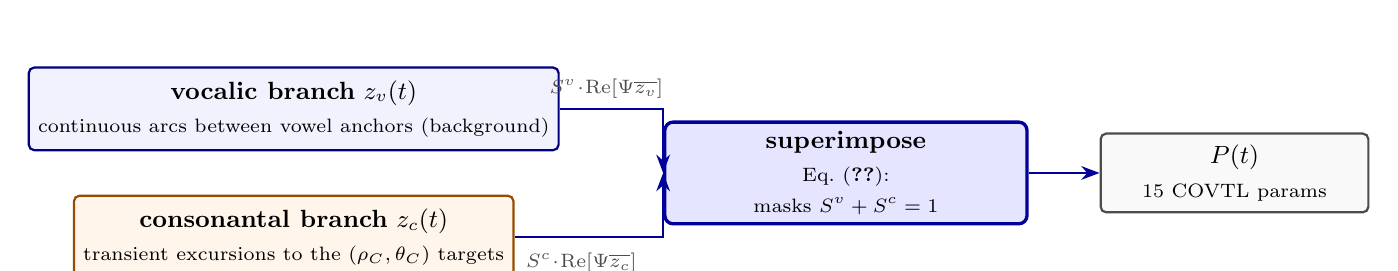
\begin{tikzpicture}[
    node distance=0.55cm and 0.9cm,
    every node/.style={font=\small},
    branch/.style={draw, rounded corners=2pt, minimum width=4.6cm, minimum height=1.05cm,
                align=center, thick},
    arrow/.style={-Stealth, thick, draw=blue!60!black},
    label/.style={font=\scriptsize\itshape, text=black!70}
]
\node[branch, fill=blue!5, draw=blue!50!black] (vocalic)
    {\textbf{vocalic branch} \(z_v(t)\)\\[1pt]
     \scriptsize continuous arcs between vowel anchors (background)};
\node[branch, fill=orange!8, draw=orange!60!black, below=of vocalic] (cons)
    {\textbf{consonantal branch} \(z_c(t)\)\\[1pt]
     \scriptsize transient excursions to the \((\rho_C, \theta_C)\) targets};

\node[draw, very thick, rounded corners=3pt, fill=blue!10, draw=blue!60!black,
      minimum width=4.6cm, minimum height=1.0cm, align=center,
      right=1.6cm of $(vocalic.east)!.5!(cons.east)$] (sup)
    {\textbf{superimpose}\\[1pt]
     \scriptsize Eq.~\eqref{eq:superposition}:\\
     \scriptsize masks \(S^v + S^c = 1\)};
\node[draw, thick, rounded corners=2pt, fill=gray!5, draw=gray!60!black,
      minimum width=3.4cm, minimum height=1.0cm, align=center,
      right=0.9cm of sup] (out)
    {\(P(t)\)\\[1pt]\scriptsize 15 COVTL params};

\draw[arrow] (vocalic.east) -- node[label, above, pos=0.45]{\(S^v\!\cdot\!\operatorname{Re}[\Psi\overline{z_v}]\)} (sup.west |- vocalic.east) -- (sup.west);
\draw[arrow] (cons.east) -- node[label, below, pos=0.45, yshift=-2pt]{\(S^c\!\cdot\!\operatorname{Re}[\Psi\overline{z_c}]\)} (sup.west |- cons.east) -- (sup.west);
\draw[arrow] (sup) -- (out);
\end{tikzpicture}%
}
\caption{The two-branch superposition of Eq.~\eqref{eq:superposition}.
Each tract parameter belongs to exactly one branch at each instant: the
consonant selector decides which.}
\label{fig:superposition}
\end{figure}

\subsection{Lightened selectors: the tongue during labials}\label{subsec:lightened}

The selectors were deliberately \emph{shortened} to increase
coarticulation, with measured justifications recorded in the source:

\begin{itemize}[leftmargin=1.5em]
\item \textbf{\texttt{b} (and \texttt{m})}: TCX/TCY removed --- the labial
      closure only needs the jaw (JA) and the lips (LD, LP). Without
      tongue parameters in the selector, \emph{the tongue follows the
      vocalic branch during the labial}; the parasitic velar contact that
      the raised \(c_1(\mathrm{TCY})\) otherwise produced disappears, with
      the labial closure itself preserved
      (\(0.000\,\mathrm{cm^2}\), lingual margins
      \(0.126\!-\!1.056\,\mathrm{cm^2}\)).
\item \textbf{\texttt{f, v}}: same lightening (TCX and TCY removed);
      the labiodental constriction is commanded by JA, JX, LP, LD only.
\item \textbf{\texttt{S, Z}}: TCY removed --- the postalveolar target
      projects a tongue center that is too high on the JD3 anatomy; by
      letting the center follow the vowel, healthy gaps of
      \(0.263\!-\!1.230\,\mathrm{cm^2}\) are obtained over the whole vowel
      set while the hushing spectrum is preserved.
\end{itemize}

The partial removal of a single parameter is not sufficient; the
lightening was validated parameter pair by parameter.

\subsection{The transition arc: an asymmetric S-curve in the plane}\label{subsec:arc}

Between a departure point \(p_d = (\rho_d, \theta_d)\) and an arrival
point \(p_a = (\rho_a, \theta_a)\), the engine does not interpolate
linearly. It sweeps an angular parameter \(\vartheta\) from
\(-\pi\) to \(0\) over \(D\) steps and blends the two projections with
the weight
\begin{equation}
r(\vartheta) \;=\; \cos^{\,p_{\mathrm{exp}}}\!\Big(\frac{\vartheta}{2}\Big),
\qquad p_{\mathrm{exp}} = 2,
\label{eq:rk}
\end{equation}
which grows from 0 to 1 as an asymmetric S-curve (slow departure, fast
arrival). The arrival term carries an extra phase \(-(\nu/K)\vartheta\)
that curves the path in the phonetic plane:
\begin{equation}
P_p(k) \;=\; c_{1,p}
\;+\; r_k\, \rho_a\, c_{0,p}
   \cos\!\big(c_{2,p} - \theta_a - \tfrac{\nu}{K}\vartheta_k\big)
\;+\; (1 - r_k)\, \rho_d\, c_{0,p}
   \cos\!\big(c_{2,p} - \theta_d\big),
\label{eq:arc}
\end{equation}
for \(k = 1 \ldots D\). This is \texttt{arc\_B} in
\texttt{polar.py} (implemented exactly as written; the arrival
\(\theta\) is \texttt{np.unwrap}ed first so that the \(\pi \to -\pi\)
wrap-around never produces a spurious \(2\pi\) jump). The curvature
constants distinguish the branches of the reference model: the consonantal
arcs use \(K_c = 10\), \(\nu = 1\), while the vocalic background uses
\(K_v = 30\) --- the vocalic handovers are much straighter. The active
\texttt{syl} engine runs with \(\nu = -1\) and a quasi-straight
\(K = 1000\) (\S\ref{sec:syltraj}); this is a notational convention
only --- \(\nu = 1\) is recovered when the cosine is written with the
opposite sign, as in Eq.~(2) of arXiv:2307.02299. The reference values
(\(K_c = 10\), \(K_v = 30\), \(\nu = 1\)) belong to the deprecated
\texttt{legacy} engine and the polar-video display.

\subsection{Clusters: per-parameter scoping}\label{subsec:clusters}

For a sequence of \(m\) consonants between two vowel anchors, the
\texttt{syl} engine builds a block of \((m+1)\) sub-arcs of
\(T_{\mathrm{cons}}\) steps each
(\texttt{build\_cluster\_pval}). The vocalic background arc between the
two anchors is computed first and fills the whole block; then, for each
sub-arc \(k\), each parameter's endpoints are set to the consonant target
\(\mathbf{C}_k\) \emph{iff} the parameter belongs to the selector of
\(\mathbf{C}_k\) --- otherwise the parameter keeps its background value at
that frame. The temporal mixing inside each sub-arc uses exactly the
reference S-curve of Eq.~\eqref{eq:rk}:
\begin{equation}
P[kT + t] \;=\; r_t \cdot \mathrm{arr} \;+\; (1 - r_t) \cdot \mathrm{dep},
\qquad t = 1 \ldots T,
\label{eq:cluster}
\end{equation}
which guarantees \(C^0\) continuity at every sub-arc boundary (zero jump,
verified by test). The active parameter set of the block is the
\emph{union} of the selectors of its consonants; a "selector frozen at
\(\theta = 0\)" never drives a parameter in a palatal context.

\subsection{Vowel-to-vowel coarticulation and the schwa waypoint}\label{subsec:vv}

\textbf{Anchors are reduced at syllable margins.} A vowel never reaches
its full target \(\rho_v\) when it is on the edge of a syllable: the
departure anchor (anticipatory) and completion anchor are scaled
(\(\delta_o = \delta_e = 0.70\) in the reference;
\(\mathrm{SYL\_COEFCEN} = 0.5\) for word-end and syllabic-onset anchors in the
\texttt{syl} engine), and a word-onset anchor is
\([0.5\,\rho_v, \theta_v]\). This is why a unstressed vowel between two
consonants is \emph{colored} by its neighbors instead of being fully
realized.

\textbf{The background never jumps.} Between two anchors the vocalic
background is a single continuous arc of \(2\,T_{\mathrm{voy}}\) steps;
an earlier conditional jump at vowel onsets was removed precisely because
it created discontinuities.

\textbf{Anti-closure routing through the schwa.} A direct polar arc
between two distant vowels can close the vocal tract mid-transition (the
superposition of the two anchor contributions sweeps through the occlusion
region --- measured on the \texttt{i--u} pair:
\(0.062\,\mathrm{cm^2}\) at mid-arc over 132 swept vowel pairs). The
engine hooks a VTL \emph{closure probe} (minimum lingual tube area at the
center of the block, on the 19-parameter resting state); when the probe
returns less than the threshold
\(0.18\,\mathrm{cm^2}\), the background arc is routed through the schwa
\(@\) as two half-arcs with exact continuity at the junctions.

\subsection{Coarticulation across word boundaries}\label{subsec:notation-coart}

The input notation is itself a coarticulation control:

\begin{itemize}[leftmargin=1.5em]
\item \texttt{.} (and \texttt{-}) is the \emph{intra-phrase syllable
      separator}: the engine coarticulates across it. Within a phrase,
      orthographic words are joined with \texttt{.} after syllabification
      by onset maximization, so \texttt{this is easy} becomes one
      connected token \texttt{Dis.iz.i.zi} --- there is \emph{no pause at
      word boundaries inside a phrase} (the syllabification rule is the
      model's answer to ``why can \emph{big.bi} be changed to
      \emph{bi.gbi}'': a single intervocalic consonant attaches to the
      next onset).
\item splitting at \texttt{.} obeys the phonotactic rule
      \textbf{C.C \(\to\) split; C.V, V.C, V.V \(\to\) merge} (the dot is
      ignored between a consonant and a vowel);
\item \emph{space} is a short inter-word pause (200\,ms default),
      \texttt{|} is the long phrase pause (320\,ms default); a comma
      produces a space and sentence punctuation produces \texttt{|};
\item the \emph{schwa principle} caps long runs: a dot is inserted after
      the first consonant of any 4+-consonant run and after the first
      vowel of any 3+-vowel run, and a vowel-less word receives a mute
      \texttt{@}.
\end{itemize}

\subsection{Nasal carry-over}\label{subsec:nasal}

Nasality coarticulates \emph{beyond} the nasal segment: velum-opening
(VO) events are extended \(20\,\mathrm{ms}\) past the end of the nasal
(\texttt{NASAL\_CARRYOVER\_MS}), and the whole VO trajectory is smoothed
with a \(20\,\mathrm{ms}\) first-order filter --- an anti-click margin
over VTL's own \(12\,\mathrm{ms}\) gesture time constant. Nasalized
vowels (\texttt{9}, \texttt{6\~{}}) receive a partial velum opening of
0.5 (vs 1.0 during nasal consonants).

%==============================================================================
\section{The syllabic trajectory engine (syltraj)}\label{sec:syltraj}
%==============================================================================

The \texttt{syl} engine (\texttt{core/syltraj.py}, the default) turns a
normalized phoneme string into the 100\,Hz polar trajectory
\(B(t)\). Its contract follows the reference COVTL specification:

\begin{enumerate}[leftmargin=1.5em]
\item \textbf{Nodes}: every phoneme carries its own polar target; no
      consonant position is ever interpolated from another consonant;
      targets are possibly adjusted by the cluster rules
      (\S\ref{subsec:context}).
\item \textbf{Anchors}: vowels only (held when isolated) plus synthetic
      \emph{vocalic} anchors: word end
      (\(\mathrm{COEFCEN}\cdot\rho\) of the last vowel), syllabic onset
      (weighted \(\rho\)), word onset (\([0.5, \theta_v]\)), and the
      terminals \([0, 0]\) that bracket the phrase.
\item \textbf{Trajectory}: a walk over consecutive anchor pairs
      (\texttt{build\_global\_pval}), emitting typed blocks
      (Table~\ref{tab:blocks}).
\end{enumerate}

\begin{table}[t]
\centering
\small
\begin{tabularx}{\textwidth}{lX}
\toprule
\textbf{Block kind} & \textbf{Content and duration} \\
\midrule
\texttt{plateau}   & vowel hold, \(T_{\mathrm{voy}}\) steps \\
\texttt{background}& vocalic arc between anchors, \(2\,T_{\mathrm{voy}}\) steps \\
\texttt{cluster}   & \(m\) consonants, \((m+1)\,T_{\mathrm{cons}}\) steps (\S\ref{subsec:clusters}) \\
\texttt{pause}     & short (\(T_{\mathrm{pause}}\)) or long (\(T_{\mathrm{pause,long}}\)) inter-word pause \\
\texttt{decay} / \texttt{attack} & fall to / rise from the previous anchor around a pending pause, \(T_{\mathrm{cons}}\) steps \\
\texttt{initial} / \texttt{terminal} & phrase bracketing from/to \([0,0]\) \\
\bottomrule
\end{tabularx}
\caption{Block types emitted by the \texttt{syl} engine. Time is counted
in gesture steps at the 100\,Hz gesture rate (1 step = 10\,ms); with the
CLI defaults \(T_{\mathrm{cons}} = 10\) steps (100\,ms),
\(T_{\mathrm{voy}} = 8\) steps (80\,ms, transition arc
\(2T_{\mathrm{voy}}\)), short pause 20 steps (200\,ms), long pause 32
steps (320\,ms).}
\label{tab:blocks}
\end{table}

The block schedule is the single time base shared by the tract and the
source: the envelope engine consumes \texttt{block\_info} directly
(\S\ref{sec:source}), a deliberate design that guarantees perfect branch
synchronization. A phrase-final vowel followed by nothing holds its
plateau (\emph{phrase-final hold}); a pause is \emph{not} a transition to
a neutral position --- the tract holds the decaying anchor.

\subsection{The orthogonal branch}\label{sec:ortho}

Three of the 19 VTL tract parameters are not commanded by the polar
model: \textbf{TS3} (tongue-side/lateral shape) and the speaker-derived
\textbf{VS} (velic). They come from the \emph{orthogonal branch}
(\texttt{core/orthogonal\_params.py}), which reads context-conditioned
targets from the \texttt{JD3.speaker} file: e.g.\ fricatives push
TS3 to \(+1.0\), laterals to \(-1.0\), closures to 0, with per-vowel
defaults looked up with the key pattern \texttt{<prefix>(<vowel>)} and a
\texttt{(a)} fallback. TS3 ramps over 10\,ms, VS over 15\,ms. The branch
is additive on TS3 and priority-based on VS, and can be disabled with
\texttt{-{}-no-ortho} (the \texttt{syl} COVTL core then works alone).

\subsection{The legacy engine}

The \texttt{legacy} engine (\texttt{-{}-engine legacy}) is the
pre-\texttt{syltraj} chain: it builds explicit superposition graphs in
the complex plane (CV, CVC, CCV graphs per syllable, executed by
\texttt{execute\_superposition\_segment}) with the reference constants
\(K_v = 30\), \(K_c = 10\), \(\nu = 1\), \(p_{\mathrm{exp}} = 2\),
scaling the consonantal branch to \(n_{\mathrm{arcs}} \cdot T \cdot
t_{\mathrm{cons}}\) and the vocalic branch to \(2T \cdot t_{\mathrm{voy}}\).
It is deprecated (a \texttt{DeprecationWarning} is emitted) and kept for
non-regression.

%==============================================================================
\section{The source model: envelopes and the glottal source}\label{sec:source}
%==============================================================================

The source branch produces the velum and glottis extensions
\(E_{\mathrm{source}}(t)\) of Eq.~\eqref{eq:global}. Its guiding
principle, stated in the code: \emph{the source envelope has no timing of
its own --- it is indexed by the articulatory events already produced by
\(B(t)\); coarticulation is inherited.}

\subsection{The three-level tag system}\label{subsec:tags}

Phonetic knowledge is described by \emph{tags}, not by raw VTL values,
through three levels (\texttt{core/tag\_system.py}):

\begin{description}[leftmargin=2em]
\item[Level A --- phonetic tags:] \texttt{voiced}, \texttt{nasal},
      \texttt{continuant}, \texttt{strident}, \texttt{aspiration},
      \texttt{place}, \texttt{manner}, \texttt{rounding}, height/depth,
      front/back, tense.
\item[Level B --- articulatory tags:] \texttt{glottal\_shape} (modal,
      voiceless, breathy, whisper, \ldots), \texttt{velum} (oral, nasal,
      nasalized), \texttt{tongue\_mode}.
\item[Level C --- control tags:] glottal opening (0--1), subglottal
      pressure (200--2000\,dPa), F0 (50--500\,Hz), aspiration strength
      (0--30\,dB), chink area (0--50).
\end{description}

A tag like \texttt{<glottal = voiceless>} is preferred to a hard-coded
value like \texttt{VO = 0.42}: phonetic tags are compiled to speaker
parameters at run time, which is what makes speaker recalibration
(JD2/JD3) possible.

\subsection{The amplitude envelope \(E(t)\) and the source timetable}

An \emph{effort} (amplitude) envelope \(E(t)\) is built from a token
reduction of the phrase (vowels V, plosives C/c, fricatives R/r, nasals
N, laterals L, silences O, final F, glide onsets y) with per-token
minimum amplitudes (V 1.0, nasals and liquids 0.3, glides 0.5). The
transitions between tokens use raised-cosine/Hanning primitives ---
e.g.\ a vowel-to-vowel junction stays at 1, a vowel-to-plosive falls as
\(\mathrm{hann}^{3}\), a plosive-to-vowel rises as \(\mathrm{hann}\).
Mapped onto the \texttt{syl} block schedule, plateaus and backgrounds get
\(E = 1\), pauses and terminals \(E = 0\), clusters a reduced
consonantal envelope, and decay/attack blocks the fading edges. The
envelope is computed at 10\,kHz and block-averaged down to 100\,Hz.

On top of \(E(t)\), a \texttt{TimedEnvelope} schedules \emph{events}
anchored to the articulatory labels (the vowel triplets
\((V_o, V, V_e)\), the consonant labels \texttt{C\_p}, \ldots) with
raised-cosine ramps. The ramp constants (in ms): attack/release 30/30,
voicing 40, velum 15, aspiration 8, F0 15, effort 20.

\subsection{Voicing, VOT and nasality}

Voicing \(V(t)\) is built per syllable from the \((V_o, V, V_e)\)
triplets: voicing starts at the first voiced consonant of the syllable
(the synthetic onset anchor \(V_o\) is purely articulatory --- silent),
stops 10\,ms before a stop coda, ramps 30\,ms in / 40\,ms out; voiceless
events then override inside obstruents. During cluster blocks, voiced
consonants (stops, nasals, liquids, voiced fricatives) carry
\(V = 1\) --- the pre-voicing bar of \texttt{/b, d, g/}.

Voice-onset time is set by place of articulation (Keating 1984; Lisker \&
Abramson 1964), in ms:

\begin{center}
\footnotesize
\begin{tabular}{@{}lccccccccc@{}}
\toprule
place & labio- & labial & dental & alveolar & post- & palatal & uvular & velar & glottal \\
 & dental & & & & alveolar & & & & \\
\midrule
VOT (ms) & 25 & 20 & 30 & 40 & 40 & 35 & 45 & 50 & 60 \\
\bottomrule
\end{tabular}
\end{center}

Nasality is the velum opening VO of \S\ref{subsec:nasal}: 1.0 during
nasal consonants, 0.5 on nasalized vowels, baseline \(-0.1\), with the
20\,ms carry-over and smoothing.

\subsection{Glottal source, pressure and effort}

The 11 glottis parameters interpolate between \textbf{presets extracted
from the \texttt{JD3.speaker} file} (\texttt{modal} --- the default, f0
102.216\,Hz, pressure 7850\,dPa; \texttt{stop}; \texttt{voiced-fricative};
\texttt{voiceless-fricative}; \texttt{whisper}; \ldots), blended by
\(V(t)\) and smoothed with a second-order critically damped Butterworth
filter (time constant 12\,ms). The subglottal pressure follows the
effort:
\begin{equation}
P_{\mathrm{sub}} \;=\; P_{\min} \;+\; \min(E, 1.5)^{1.2}\,
\big(P_{\max} - P_{\min}\big),
\qquad P_{\max} = 8\,000\,\mathrm{dPa},
\label{eq:pressure}
\end{equation}
with a phonation floor of \(3\,000\,\mathrm{dPa}\) while voicing is on
and a pre-voicing regime during voiced closures (pressure 1800\,dPa,
relative amplitude clipped to 0.10--0.18). The pulmonary-effort variant
zeroes the effort on plosive occlusions (5\,ms smoothing) and takes the
maximum of the effort, \(60\,\%\) of the pre-voicing level and
\(50\,\%\) of nasality before smoothing (10\,ms).

A per-vowel effort gain compensates the intrinsic intensity deficit of
high vowels: \texttt{i, u, e} \(\times 1.5\), \texttt{y}
\(\times 1.3\), \texttt{2} \(\times 1.2\) on their plateaus
(\(\approx +3\,\mathrm{dB}\)).

\subsection{F0: declination and micro-prosody}

The default F0 is the JD3 speaker default \(102.216\,\mathrm{Hz}\). Each
phrase receives a French-style \textbf{declination} (Jun \& Fougeron
2002): \(+3\,\%\) at onset, \(-15\,\%\) at the end, linear in between;
phrases are detected as voiced spans separated by more than 200\,ms of
silence. Superimposed on it, a \textbf{micro-prosody} couples F0 to the
effort envelope:
\begin{equation}
F0(t) \;=\; F0_{\mathrm{base}} \;+\; k_E\,\big(E(t) - \overline{E}\big),
\qquad k_E = 10\,\mathrm{Hz},
\end{equation}
clamped to \([40, 600]\,\mathrm{Hz}\), with the last voiced value held
through unvoiced spans.

%==============================================================================
\section{The multi-speaker registry and the language pack}\label{sec:multispeaker}
%==============================================================================

Since v1.1.0 the package carries five speakers and six languages.
Both selectors follow the same design: a \emph{registry} on disk is
the single source of truth, and one reversible command swaps the
installed state; \texttt{restore} always returns to a bit-exact
previous state.

\subsection{The speaker registry}

The directory \texttt{vtl\_synth/data/speakers/} holds
\texttt{registry.json} (one entry per speaker: file names,
\texttt{f0\_default}, description, SHA-256 of both files), the
\texttt{ACTIVE\_SPEAKER} marker, the five \texttt{.speaker} files and
their \texttt{\_constants.py} sources. The installed
\texttt{core/constants.py} is always a bit-exact copy of a registry
source, so its hash identifies the speaker.

\begin{center}
\small
\begin{tabular}{@{}lllrl@{}}
\toprule
\textbf{name} & \textbf{origin} & \textbf{sex} &
\textbf{f0\_default (Hz)} & \textbf{vowel targets} \\
\midrule
\texttt{jd3} & VTL 2.4 reference & male & 102.216 & follows the language pack \\
\texttt{s1}  & DVTD subject 1 (MRI) & male & 114.908 & native (v3 constants) \\
\texttt{s2}  & DVTD subject 2 (MRI) & female & 181.008 & native (v3 constants) \\
\texttt{m01} & official VTL 2.4 (Option A) & male & 120.000 & native (v3 constants) \\
\texttt{w02} & official VTL 2.4 (Option A) & female & 232.458 & native (v3 constants) \\
\bottomrule
\end{tabular}
\end{center}

A switch coordinates four layers: the installed \texttt{constants.py}
(geometry, glottis, \texttt{f0\_default}), the \texttt{.speaker} file
read by the orthogonal branch at each call, the shared speaker
resource of the \texttt{vocaltractlab-cython} wheel (effective in the
next process), and the per-speaker regression baselines
(\texttt{regression\_baselines\_\{s1,s2,m01,w02\}.json}, regenerated by
\texttt{scripts/regen\_baselines.py}).

\begin{lstlisting}[style=shell]
python install_speaker.py list            # speakers + active one
python install_speaker.py install s2      # 7-step swap + smoke test
python install_speaker.py restore         # back to jd3 (bit-exact)
python install_speaker.py status          # hashes, layer coherence
\end{lstlisting}

Every \texttt{install} runs a smoke test in a fresh subprocess and
rolls back automatically on any error; every synthesis announces the
four layers (constants, ortho, audio wheel, video) and warns on any
disagreement. Provenance of the five speakers, the two adaptation
chains and the defect catalogue are documented in
\texttt{docs/speakers.pdf}.

\subsection{The language pack}

\texttt{setup\_lang.py} manages a delimited LANG SECTION
(\texttt{VOWEL\_TARGETS}, \texttt{VOWEL\_EFFORT\_GAIN},
\texttt{ACTIVE\_LANG}) inside the installed \texttt{constants.py},
plus per-language g2p profiles, lexicons (Wikipron) and prosodic
timings:

\begin{lstlisting}[style=shell]
python setup_lang.py install --lang fr    # install + activate
python setup_lang.py setlang en|fr|es|de|it|pt
python setup_lang.py calibrate fr --in-situ   # JD3 only (guard)
python setup_lang.py verify               # in-situ LPC check
python setup_lang.py restore --purge      # full uninstall
\end{lstlisting}

Two invariants matter for day-to-day use. \textbf{Only JD3 follows
the pack}: the per-language vowel targets are calibrated in situ on
JD3, and the language-management commands carry a guard that
(re)installs jd3 before touching the LANG SECTION; the other speakers
are used with their native targets. \textbf{Per-call override}: the
CLI flag \texttt{-l} / \texttt{-{}-lang} selects the language of a
single call without switching the installation. Installation,
calibration, verification scores and troubleshooting are documented
in \texttt{docs/language\_pack.pdf}; the expressive-prosody option
(\texttt{-{}-expressive}) and its interaction with the registry in
\texttt{docs/expressive\_prosody.pdf}.

%==============================================================================
\section{Architecture and data flow}\label{sec:architecture}
%==============================================================================

The package is organized into five subpackages:

\begin{description}[leftmargin=2em]
\item[\texttt{vtl\_synth.core}] the synthesis engine: notation/parsing,
      phoneme tables, the polar model, the trajectory engines, the
      envelope/source modules, the \texttt{Pipeline} orchestrator, and
      the speaker registry resolver (\texttt{speaker\_registry.py}).
\item[\texttt{vtl\_synth.cli}] the \texttt{vtl-synth} entry point with
      the subcommands \texttt{run}, \texttt{text-to-wav},
      \texttt{tract-to-mp4}, \texttt{polar-build},
      \texttt{polar-video}, \texttt{inspect}, \texttt{plot-tract}.
\item[\texttt{vtl\_synth.vtl}] the VocalTractLab API facade
      (\texttt{api.py}) over the \texttt{vocaltractlab-cython} wheel.
\item[\texttt{vtl\_synth.video}] the sagittal renderer
      (\texttt{renderer.py}: SVG frames \(\to\) PNG), the MP4 encoder
      (\texttt{encoder.py}: ffmpeg H.264/AAC), the parameter figure
      tool (\texttt{tract\_figure.py}), and the polar-figure module
      (\texttt{polar\_video.py}: two-branch reconstruction,
      dual-panel composition).
\item[\texttt{vtl\_synth.utils}] the grapheme-to-phoneme modules
      (English \texttt{g2p.py} on CMUdict; the five language-pack
      profiles), the language-profile layer (\texttt{setlang.py},
      \texttt{lexicon\_loader.py}) and the prosody add-ons
      (\texttt{chunking.py}, \texttt{prosody\_f0.py}).
\item[\texttt{vtl\_synth.data.speakers}] the speaker registry:
      \texttt{registry.json}, the \texttt{ACTIVE\_SPEAKER} marker,
      the five \texttt{.speaker} files and their
      \texttt{\_constants.py} sources (\S\ref{sec:multispeaker}).
\end{description}

\subsection{Data flow}

\begin{center}
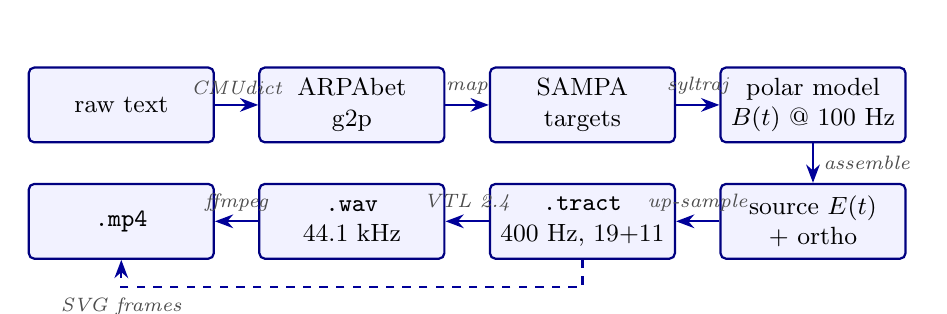
\begin{tikzpicture}[
    node distance=0.5cm and 0.55cm,
    every node/.style={font=\small},
    box/.style={draw, rounded corners=2pt, minimum width=2.35cm, minimum height=0.95cm,
                align=center, fill=blue!5, draw=blue!50!black, thick},
    arrow/.style={-Stealth, thick, draw=blue!60!black},
    label/.style={font=\scriptsize\itshape, text=black!70}
]
\node[box] (text) {raw text};
\node[box, right=of text] (g2p) {ARPAbet\\g2p};
\node[box, right=of g2p] (sampa) {SAMPA\\targets};
\node[box, right=of sampa] (polar) {polar model\\$B(t)$ @ 100 Hz};

\node[box, below=of polar] (src) {source $E(t)$\\+ ortho};
\node[box, left=of src] (tract) {\texttt{.tract}\\400 Hz, 19+11};
\node[box, left=of tract] (wav) {\texttt{.wav}\\44.1 kHz};
\node[box, left=of wav] (mp4) {\texttt{.mp4}};

\draw[arrow] (text) -- node[label, above]{CMUdict} (g2p);
\draw[arrow] (g2p) -- node[label, above]{map} (sampa);
\draw[arrow] (sampa) -- node[label, above]{syltraj} (polar);
\draw[arrow] (polar) -- node[label, right]{assemble} (src);
\draw[arrow] (src) -- node[label, above]{up-sample} (tract);
\draw[arrow] (tract) -- node[label, above]{VTL 2.4} (wav);
\draw[arrow] (wav) -- node[label, above]{ffmpeg} (mp4);
\draw[arrow, dashed] (tract.south) -- ++(0,-0.35) -| (mp4.south)
    node[label, below, midway]{SVG frames};
\end{tikzpicture}
\end{center}

Each stage of the chain:

\begin{enumerate}[leftmargin=1.5em]
\item \textbf{g2p}: English text \(\to\) connected engine SAMPA tokens
      (\S\ref{sec:notation}); or direct SAMPA with
      \texttt{-{}-phonetic}.
\item \textbf{Parse \& normalize}: Unicode/IPA normalization, longest-match
      tokenization, phrase splitting on \texttt{|}, syllable structure.
\item \textbf{\(B(t)\)}: the \texttt{syl} engine builds the 100\,Hz polar
      trajectory block by block (\S\ref{sec:syltraj}), projected through
      Eq.~\eqref{eq:computeP} into the 15 COVTL parameters.
\item \textbf{Source}: the envelope \(E(t)\), voicing \(V(t)\), velum
      VO/VS, glottis trajectory and F0 (\S\ref{sec:source}), all indexed
      by the block schedule; the orthogonal branch adds TS3/VS
      (\S\ref{sec:ortho}).
\item \textbf{Assemble}: the 15 COVTL parameters are scattered into the
      19-parameter VTL vector (VS at index 6, VO at 7; TS3 additive;
      TRX/TRY left at 0 --- VTL drives them), the glottis block is
      appended, and everything is linearly up-sampled 100
      \(\to\) 400\,Hz into the \texttt{.tract} file.
\item \textbf{VTL synthesis}: each tract state \(\to\) area function
      (40 tube sections, JD3 anatomy) \(\to\) aerodynamic-acoustic
      simulation \(\to\) 110 audio samples per state at 44.1\,kHz.
\item \textbf{Video}: every video frame is exported as an SVG of the
      sagittal cross-section by VTL itself, rasterized to PNG, and
      encoded with the bundled ffmpeg.
\end{enumerate}

\begin{callout}[Three sampling rates]
\begin{itemize}[leftmargin=1.5em]
\item \textbf{Model rate}: 100\,Hz (gesture step 10\,ms) --- the polar
      trajectory and the envelopes.
\item \textbf{Tract rate}: 400\,Hz (\texttt{.tract}) --- 19 tract + 11
      glottis parameters per frame, 2.5\,ms hop.
\item \textbf{Audio rate}: \(44\,100\,\mathrm{Hz}\) --- 110 audio samples
      per tract state (\texttt{.wav}, PCM 16-bit mono).
\end{itemize}
\end{callout}

%==============================================================================
\section{CLI reference}\label{sec:cli}
%==============================================================================

The \texttt{vtl-synth} command exposes seven subcommands:
\texttt{run}, \texttt{text-to-wav}, \texttt{tract-to-mp4},
\texttt{polar-build}, \texttt{polar-video}, \texttt{inspect} and
\texttt{plot-tract}. The engine options (COVTL model parameters) are
shared by \texttt{run} and \texttt{text-to-wav}:

\begin{center}
\small
\begin{tabularx}{\textwidth}{lX}
\toprule
\textbf{Engine flag} & \textbf{Description} \\
\midrule
\texttt{-{}-phonetic}        & input is already engine SAMPA (skip g2p) \\
\texttt{-l, -{}-lang CODE}   & language for this call only (default: the active language of the pack, \S\ref{sec:multispeaker}) \\
\texttt{-{}-tcons MS}        & consonant (sub-arc) duration, default: active language profile (en: \textbf{100\,ms}) \\
\texttt{-{}-tvoy MS}         & vowel gesture duration, default: active language profile (en: \textbf{80\,ms}) \\
\texttt{-{}-tpause MS}       & short inter-word pause (space), default: active language profile (en: \textbf{200\,ms}) \\
\texttt{-{}-tpause-long MS}  & long phrase pause (\texttt{|}), default: active language profile (en: \textbf{320\,ms}) \\
\texttt{-f0, -{}-f0 HZ}      & fundamental frequency, default: \texttt{f0\_default} of the active speaker (102.216\,Hz for JD3) \\
\texttt{-s, -{}-speaker}     & speaker name, default \texttt{JD3} \\
\texttt{-{}-expressive} / \texttt{-{}-no-expressive} & expressive prosody (breathing + sculpted F0) / monotone declination (default); see \texttt{docs/expressive\_prosody.pdf} \\
\texttt{-{}-no-ortho}        & disable the orthogonal branch (TS3/VS) \\
\texttt{-{}-engine \{syl,legacy\}} & trajectory engine, default \texttt{syl} \\
\bottomrule
\end{tabularx}
\end{center}

\subsection{run --- all-in-one synthesis}

\begin{lstlisting}[style=shell]
vtl-synth run "this is easy for us" [options]
\end{lstlisting}

Runs the full pipeline: text \(\to\) \texttt{.tract} \(\to\) \texttt{.wav}
\(\to\) \texttt{.mp4} (+ the SAMPA transcript \texttt{.txt}).

\begin{center}
\small
\begin{tabularx}{\textwidth}{lX}
\toprule
\textbf{Flag} & \textbf{Description} \\
\midrule
\texttt{-o, -{}-output-dir} & output directory (default: \texttt{./out}) \\
\texttt{-{}-label}          & filename stem (default: derived from the text) \\
\texttt{-{}-no-video}       & skip MP4 rendering \\
\texttt{-{}-polar}          & also write the \texttt{.polar} file and render the dual-panel video (tract | polar figure); see \texttt{docs/polar\_visualization.pdf} \\
\texttt{-{}-fps}            & video frame rate (default: 25) \\
\texttt{-{}-scale}          & pixels per SVG unit (default: 2 \(\to\) 960\(\times\)840) \\
\bottomrule
\end{tabularx}
\end{center}

\begin{lstlisting}[style=shell]
# Direct phonetic input (no g2p): syllables '.', short pause ' ', long '|'
vtl-synth run --phonetic "ba da ga | iowa a g" -o ./out

# Slower, more coarticulated speech
vtl-synth run "this is easy for us" -o ./out --tcons 140 --tvoy 110

# Audio only
vtl-synth run "hello world" -o ./out --no-video

# French, expressive prosody (breathing + sculpted F0)
vtl-synth run "bonjour le monde" -l fr --expressive -o ./out --no-video

# Dual-panel polar video (en/jd3)
vtl-synth run --polar "this is easy for us" -l en -o ./out --label polar_demo_en
\end{lstlisting}

\subsection{text-to-wav --- audio-only synthesis}

\begin{lstlisting}[style=shell]
vtl-synth text-to-wav "hello world" -o ./out
\end{lstlisting}

Same engine path as \texttt{run}, stops after the \texttt{.wav}.

\subsection{tract-to-mp4 --- re-render a video}

\begin{lstlisting}[style=shell]
vtl-synth tract-to-mp4 <tract> [<wav>] [-o output.mp4] [--fps 25] [--scale 2]
\end{lstlisting}

Re-renders the sagittal video from an existing \texttt{.tract}; when the
\texttt{.wav} is omitted it is re-synthesized from the tract. Useful to
change resolution or frame rate without re-running the model.

\subsection{polar-build / polar-video --- the polar figure}

\begin{lstlisting}[style=shell]
# .polar only, from a phrase in the internal notation
vtl-synth polar-build "ba.da.ga" -o out/ba.polar --tcons 160

# Dual-panel video from existing files
vtl-synth polar-video out/x.tract --polar out/x.polar out/x.wav -o out/x.mp4
\end{lstlisting}

\texttt{polar-build} reconstructs the two 100\,Hz polar trajectories
(vocalic branch / consonantal branch) of a phrase and writes the JSON
\texttt{.polar} side-car; \texttt{polar-video} composes the
dual-panel MP4 (sagittal view | polar figure, 25\,Hz) from a
\texttt{.tract}, a \texttt{.polar} and a \texttt{.wav}. The
reconstruction, the file format and the rendering are documented in
\texttt{docs/polar\_visualization.pdf}.

\subsection{inspect --- tract inspector}

\begin{lstlisting}[style=shell]
vtl-synth inspect ./out/this_is_easy_for_us.tract --states 2 --ranges
\end{lstlisting}

Prints the shape, rate and duration of the tract sequence, the first/last
N states as per-parameter tables, and with \texttt{-{}-ranges} the
min/max/mean of each of the 19 tract parameters.

\subsection{plot-tract --- graphical inspector}

\begin{lstlisting}[style=shell]
vtl-synth plot-tract ./out/this_is_easy_for_us.tract --which all -o ./out/tract.png
vtl-synth plot-tract ./out/this_is_easy_for_us.tract --params JX JA TTX TTY --ranges
\end{lstlisting}

Draws the 400\,Hz trajectory of every tract parameter into a PNG figure
(shared time axis, one subplot per parameter); \texttt{-{}-which all} adds
the glottis f0 and pressure, \texttt{-{}-params} restricts the tract
block, \texttt{-{}-ranges} prints the \texttt{inspect} table. Requires
the optional \texttt{plot} extra (\texttt{pip install ".[plot]"}).

%==============================================================================
\section{Python API reference}\label{sec:api}
%==============================================================================

\subsection{Pipeline --- high-level orchestrator}

\begin{lstlisting}[style=python]
from vtl_synth import Pipeline

pipe = Pipeline(
    f0_hz=102.216,        # JD3 default; per-phrase declination applied
    speaker="JD3",
    engine="syl",         # 'syl' (recommended) or 'legacy'
    use_orthogonal=True,  # TS3/VS orthogonal branch
    t_cons_ms=100.0,      # consonant sub-arc duration
    t_voy_ms=80.0,        # vowel gesture duration
    pause_short_ms=200.0, # inter-word pause
    pause_long_ms=320.0,  # end-of-sentence pause
)

result = pipe.run("this is easy for us", output_dir="./out")
print(result.sampa)               # 'Dis.iz.i.zi.fOR.@s'
print(result.tract_path, result.n_frames, result.duration_s)

# phonetic input, audio only
result = pipe.text_to_wav("ba da ga | iowa a g",
                          output_dir="./out/phon", use_g2p=False)
\end{lstlisting}

The \texttt{PipelineResult} dataclass exposes \texttt{sampa},
\texttt{phrases}, the artifact paths (\texttt{tract\_path},
\texttt{wav\_path}, \texttt{mp4\_path}), \texttt{n\_frames}
(at 400\,Hz), \texttt{duration\_s} and \texttt{warnings}.

\subsection{Video re-rendering}

\begin{lstlisting}[style=python]
info = Pipeline.tract_to_mp4(
    tract_path="./out/this_is_easy_for_us.tract",
    wav_path="./out/this_is_easy_for_us.wav",
    out_path="./out/regenerated.mp4",
    fps=25, scale=2,
)
\end{lstlisting}

This does \emph{not} re-run the model: it parses the tract sequence,
renders one SVG frame per video frame and encodes with ffmpeg.

\subsection{Engine and VTL APIs}

The full engine API (63 public symbols) is available from
\texttt{vtl\_synth.core}: the orchestrators
(\texttt{Pipeline}, \texttt{build\_phrase\_tract}, \texttt{text\_to\_tract}),
the polar model (\texttt{compute\_P}, \texttt{arc\_B}, \texttt{polar\_arc},
\texttt{project\_covtl}, \texttt{superimpose}), the trajectory engines
(\texttt{build\_phrase\_pval}, \texttt{build\_global\_pval}), the
envelope/source modules (\texttt{TimedEnvelope}, \texttt{FeatureTimer},
\texttt{build\_glottis\_trajectory}), the constants
(\texttt{VOWEL\_TARGETS}, \texttt{CONSONANT\_TARGETS}, \texttt{CO\_VTL},
\texttt{CO}) and the assembly layer (\texttt{AssembleTract},
\texttt{write\_tract\_file}).

\noindent\begin{minipage}{\linewidth}
\begin{lstlisting}[style=python]
from vtl_synth.vtl.api import (synthesize_to_wav, render_tract_svg,
                               get_vtl_info, get_vowel_shape,
                               get_transfer_function)

info = get_vtl_info()
# {'version': ..., 'speaker': 'JD3', 'sr_audio': 44100,
#  'sr_internal': 400.0, 'n_tract_params': 19,
#  'n_glottis_params': 11, 'n_samples_per_state': 110,
#  'n_tube_sections': 40, ...}

synthesize_to_wav("./out/this_is_easy_for_us.tract",
                  "./out/resynthesized.wav")
\end{lstlisting}
\end{minipage}

%==============================================================================
\section{Input notation and grapheme-to-phoneme conversion}\label{sec:notation}
%==============================================================================

\subsection{Engine SAMPA inventory}

\begin{itemize}[leftmargin=1.5em]
\item \textbf{Vowels}: \texttt{a e i o u y E O @ 2 6 9}
      (12 targets, Table~\ref{tab:vowels});
\item \textbf{Consonants}: \texttt{p b t d k g f v s z S Z T D tS dZ m n
      J l L R j w h \turnh{} C X} (canonical voiced forms of
      Table~\ref{tab:cons} plus their voiceless partners; \texttt{R}
      is the only rhotic --- a spelled \texttt{r} in the input is
      normalized to \texttt{R} by \texttt{notation.py});
\item \textbf{Separators}: \texttt{.} syllable break (coarticulated),
      space short pause, \texttt{|} long pause; \texttt{\~{}} marks
      nasality.
\end{itemize}

\subsection{English text rules}

With English text input (the default), the bundled g2p applies:

\begin{enumerate}[leftmargin=1.5em]
\item CMUdict lookup of each word (first pronunciation), stress digits
      stripped;
\item ARPAbet \(\to\) engine SAMPA mapping (Table~\ref{tab:arpa});
\item syllabification by onset maximization: the vowel closes the
      nucleus, a single intervocalic consonant attaches to the next
      onset, longer clusters split before the last consonant, word-final
      consonants form the coda;
\item the words of a phrase are joined with \texttt{.} into connected
      tokens --- the engine coarticulates across word boundaries
      (\S\ref{subsec:notation-coart}).
\end{enumerate}

Punctuation: sentence-ending punctuation (\texttt{.!?;:}) becomes the
long phrase pause \texttt{|}; a comma or dash becomes the short inter-word
pause. Unknown words that are already valid engine SAMPA
(\texttt{is\_sampa\_token}) are passed through verbatim; other unknown
words are kept with a warning.

\begin{table}[t]
\centering
\small
\begin{tabular}{@{}llp{5.9cm}@{}}
\toprule
\textbf{ARPAbet} & \textbf{SAMPA} & \textbf{Note} \\
\midrule
P B T D K G & p b t d k g & direct (voiceless resolves to voiced target) \\
CH, JH & tS, dZ & affricates \\
F V S Z SH ZH & f v s z S Z & direct \\
TH, DH & T, D & dental fricatives --- engine targets exist \\
HH & h & direct \\
M N NG & m n J & nasals; \texttt{NG}\(\to\)\texttt{J} is a documented
  compromise: the English velar nasal [ŋ] is mapped to the derived
  dorsal node (neither \texttt{N} nor \texttt{J} carries a closure
  target, Table~\ref{tab:cons}) \\
L R W Y & l R w j & R is the uvular of the engine inventory \\
AA AE & a & AE merges to \texttt{a} \\
AH & @ & schwa \\
AO & O & \\
EH EY & E, e & \\
IH IY & i, i & quantity not distinguished \\
OW & o & \\
UH UW & u, u & quantity not distinguished \\
AW AY OY ER & a\,w,\ a\,j,\ O\,j,\ @\,R & diphthongs/rhotic \(\to\) key sequences \\
\bottomrule
\end{tabular}
\caption{ARPAbet \(\to\) engine SAMPA mapping
(\texttt{ARPA\_TO\_SAMPA}, \texttt{core/phonemes.py}).}
\label{tab:arpa}
\end{table}

%==============================================================================
\section{File formats reference}\label{sec:formats}
%==============================================================================

\subsection{\texttt{.tract} --- tract sequence at 400\,Hz}

Plain-text file: comment lines starting with \texttt{\#}, a fixed header
(sample rate, parameter counts and names, frame count), then one line per
frame with the 19 tract + 11 glottis values
(\texttt{\%.6f}):

\begin{lstlisting}[style=verbatim]
# VTL tract sequence file
# version: 1
# sample_rate: 400
# n_tract_params: 19
# n_glottis_params: 11
# n_frames: 952
# tract_param_names: HX HY JX JA LP LD VS VO TCX TCY TTX TTY TBX TBY
#                    TRX TRY TS1 TS2 TS3
# glottis_param_names: f0 pressure x_bottom x_top chink_area lag rel_amp
#                    double_pulsing pulse_skewness f0_flutter
#                    aspiration_strength
# ---
<frame 0: 19 tract values, then 11 glottis values>
...
\end{lstlisting}

The 19 tract parameters: hyoid \texttt{HX HY}, jaw \texttt{JX JA}, lips
\texttt{LP LD}, velopharyngeal port \texttt{VS VO} (extensions), tongue
center \texttt{TCX TCY}, tongue tip \texttt{TTX TTY}, tongue base
\texttt{TBX TBY}, tongue root \texttt{TRX TRY} (auto-driven, kept at 0),
tongue shape \texttt{TS1 TS2 TS3}. The 11 glottis parameters:
\texttt{f0} (Hz), \texttt{pressure} (dPa), \texttt{x\_bottom},
\texttt{x\_top}, \texttt{chink\_area} (posterior opening/breathiness),
\texttt{lag}, \texttt{rel\_amp}, \texttt{double\_pulsing},
\texttt{pulse\_skewness}, \texttt{f0\_flutter} (\%),
\texttt{aspiration\_strength} (dB).

The reader is \texttt{read\_tract} (\texttt{vtl\_synth.video.renderer});
it parses \texttt{\# sample\_rate:} and expects at least 19 columns.

\subsection{\texttt{.wav}, \texttt{.mp4}, \texttt{.txt}}

\begin{itemize}[leftmargin=1.5em]
\item \texttt{.wav}: PCM 16-bit mono at \(44\,100\,\mathrm{Hz}\),
      peak-normalized to \(0.9\) full scale by the pipeline.
\item \texttt{.mp4}: H.264 (\texttt{yuv420p}) + AAC; default
      960\(\times\)840 at 25\,fps (\texttt{-{}-scale 2}). The upper panel
      is the sagittal cross-section exported by VTL as SVG; the audio
      track is muxed by ffmpeg (\texttt{-shortest}).
\item \texttt{.txt}: the engine SAMPA transcript actually synthesized
      (e.g.\ \texttt{Dis.iz.i.zi.fOR.@s}) --- the audit trail of the g2p.
\item \texttt{.polar} (optional, \texttt{-{}-polar}): JSON side-car
      carrying the two 100\,Hz polar trajectories (vocalic /
      consonantal, \texttt{null} while a branch is inactive) and the
      phoneme timing; consumed by the dual-panel video
      (\texttt{docs/polar\_visualization.pdf}).
\end{itemize}

%==============================================================================
\section{Worked example: ``this is easy for us''}\label{sec:example}
%==============================================================================

This section walks through the real output of the demo phrase in the
default configuration (speaker jd3, language en; all numbers measured
on the artifacts of a default run).

\subsection{g2p output}

\begin{lstlisting}[style=verbatim]
word   ARPAbet (CMUdict)   engine token
this   DH IH1 S            Dis
is     IH1 Z               iz
easy   IY1 Z IY0           i.zi
for    F AO1 R             fOR
us     AH1 S               @s
\end{lstlisting}

The words of the phrase are connected with \texttt{'.'}, giving the
single engine token \texttt{Dis.iz.i.zi.fOR.@s}. Note the
resyllabifications
(\emph{is\ easy} \(\to\) \texttt{iz.i.}, \emph{easy} split
\texttt{i.zi}): one coarticulated phrase, no pause at the orthographic
word boundaries. The full SAMPA transcript written to \texttt{.txt}:
\texttt{Dis.iz.i.zi.fOR.@s}.

\subsection{Tract sequence}

\begin{lstlisting}[style=verbatim]
shape     : (952, 30)  (11 glottis cols)
rate      : 400 Hz
duration  : 2.380 s
\end{lstlisting}

952 frames at 2.5\,ms hop. The first and last frames are the resting
state --- the projection of the phrase-terminal anchors \([0, 0]\) is the
center line of Table~\ref{tab:co}, e.g.\ \texttt{HX = 0.722},
\texttt{JA = $-$3.371}, \texttt{TCX = 1.091}.

\subsection{Audio and video}

\begin{lstlisting}[style=verbatim]
wav : PCM 16-bit, 1 channel, 44100 Hz, 104720 frames, 2.3746 s
      peak 90.00 % FS (pipeline normalization), RMS 7.6 % FS
mp4 : h264 (High), yuv420p, 960x840, 25 fps, 2.40 s
      + aac 44100 Hz mono; 239,001 bytes
\end{lstlisting}

The video and audio durations agree to within one video frame
(2.40 vs 2.37\,s), confirming the sync (each frame decimates the 400\,Hz
tract sequence by \(400/25 = 16\) frames).

%==============================================================================
\section{Differences with the vtl-pipeline reference repository}\label{sec:differences}
%==============================================================================

The \href{https://github.com/FBerthommier/vtl-pipeline}{vtl-pipeline}
reference repository chains VTL-native stages
(text \(\to\) \texttt{.seg} \(\to\) \texttt{.ges} \(\to\) tract
\(\to\) wav/mp4) through a ctypes binding to
\texttt{libVocalTractLabApi}. covtl-pipeline shares its packaging and CLI
layout but synthesizes the tract sequence \textbf{directly} with the
Berthommier COVTL model:

\begin{center}
\small
\begin{tabularx}{\textwidth}{lXX}
\toprule
 & \textbf{vtl-pipeline (reference)} & \textbf{covtl-pipeline} \\
\midrule
Tract generation & VTL segment \(\to\) gestural score & COVTL polar model, no \texttt{.seg}/\texttt{.ges} \\
Coarticulation & VTL gesture blending & selector superposition (\S\ref{sec:coart}) \\
Targets & VTL shape library & \((\rho,\theta)\) plane (\S\ref{sec:polar}) \\
VTL backend & ctypes \texttt{.so} + Krug wheel & \texttt{vocaltractlab-cython} wheel \\
Input & English text & English text or SAMPA (\texttt{-{}-phonetic}) \\
\bottomrule
\end{tabularx}
\end{center}

Consequences: no \texttt{.seg}/\texttt{.ges} files exist in the output
(\texttt{inspect} rejects them with an explanatory message), no manual
DLL/library management is needed, and the articulatory trajectory is
fully transparent --- every 100\,Hz model sample derives from the
documented equations of \S\ref{sec:polar}--\S\ref{sec:coart}.

%==============================================================================
\section{Limitations and known issues}\label{sec:limitations}
%==============================================================================

\begin{itemize}[leftmargin=1.5em]
\item \textbf{English phoneme approximations.} The engine works on a
      French-style SAMPA inventory: \texttt{R} is uvular (English rhotics
      are approximated), \texttt{AE/AH} merge to \texttt{a/@}, quantity
      contrasts (\texttt{IH/IY}, \texttt{UH/UW}) are not distinguished,
      and \texttt{ER} becomes the sequence \texttt{@ R}. Dental
      fricatives \texttt{TH/DH} do have engine targets (\texttt{T/D} at
      \(271^\circ\)).
\item \textbf{Fixed gesture durations.} One \texttt{-{}-tcons}/\texttt{-{}-tvoy}
      pair applies to the whole utterance; there is no per-phoneme
      duration model, no stress-weighted durations and no word-final
      lengthening beyond the phrase-final hold.
\item \textbf{Derived places.} \texttt{N} and \texttt{J} have empty
      selectors (derived velar/dorsal places); \texttt{h} is a
      near-neutral target driven by the source.
\item \textbf{Legacy engine deprecated.} \texttt{-{}-engine legacy} emits
      a \texttt{DeprecationWarning} and is kept only for non-regression.
\item \textbf{Video renderer.} The SVG \(\to\) PNG rasterizer is a
      lightweight polyline renderer built on Pillow (no cairo
      dependency); complex SVG features beyond the VTL sagittal output
      are not supported.
\item \textbf{Python 3.9 compatibility mode.} With
      \texttt{vocaltractlab-cython==0.0.13}, the four analysis helpers
      added in 0.0.16+ (\texttt{get\_cross\_sections},
      \texttt{get\_centerline}, \texttt{get\_outlines},
      \texttt{get\_active\_speaker}) raise a clear error; synthesis and
      video are unaffected.
\end{itemize}

%==============================================================================
\section{Developer guide}\label{sec:dev}
%==============================================================================

\subsection{Package layout}

\begin{lstlisting}[style=verbatim]
covtl-pipeline/
|-- pyproject.toml             PEP 621 metadata (Python >= 3.9), GPL-3.0-or-later
|-- LICENSE                    GPL-3.0 full text
|-- THIRD_PARTY_NOTICES.md     upstream author credits
|-- README.md, INSTALL.md, CHANGELOG.md
|-- launch.bat                 Windows quick-launch script
|-- install_speaker.py         speaker selector (list/install/restore/status)
|-- setup_lang.py              language selector (install/setlang/...)
|-- lang_pack/                 language pack source tree, lexicons, manual
|-- regression_baselines.json           E2E baselines, speaker jd3
|-- regression_baselines_{s1,s2,m01,w02}.json  per-speaker baselines
|-- examples/                  demo.py, demo_prosody.py
|-- scripts/                   regen_baselines.py, calibrate_fine_v2.py,
|                              f0_report.py, check_vowel_area.py
|-- tests/                     lightened quick suite (see below)
|-- docs/                      the five manuals (LaTeX + PDF)
`-- vtl_synth/
    |-- __init__.py            public API exports (Pipeline, ...)
    |-- core/                  engine modules (model, trajectories,
    |                          source, speaker_registry)
    |-- cli/main.py            vtl-synth entry point (7 subcommands)
    |-- video/                 renderer, encoder, tract_figure, polar_video
    |-- vtl/api.py             VocalTractLab API facade
    |-- utils/                 g2p, language profiles, prosody add-ons
    `-- data/
        |-- vtl_binaries/JD3.speaker     package speaker data
        `-- speakers/          registry.json, ACTIVE_SPEAKER,
                               *.speaker, *_constants.py (5 speakers)
\end{lstlisting}

\subsection{Running the tests}

\begin{lstlisting}[style=shell]
pip install -e ".[dev]"
pytest -v                                     # quick suite
pytest tests/test_regression_baselines.py     # per-speaker E2E baselines
pytest tests/test_speaker_registry.py         # registry integrity
\end{lstlisting}

The repository ships a lightened quick suite: end-to-end
non-regression against the per-speaker baseline files
(\texttt{regression\_baselines.json} for jd3 and one baseline file
per other speaker), speaker-registry integrity, and fast CLI/g2p unit tests. The full
development battery (polar model, syltraj structure, notation/parsing,
glottal classification, expressive prosody, multi-language g2p, tract
figure; 112 tests in 10 modules on the reference development
installation) runs from the development tree with
\texttt{pytest -m "not slow"}.

\subsection{Extending the model}

\begin{itemize}[leftmargin=1.5em]
\item \textbf{New phoneme target}: add the \((\rho, \theta)\) entry (and
      selector) to \texttt{CONSONANT\_TARGETS} or to
      \texttt{VOWEL\_TARGETS} in \texttt{core/constants.py} --- the
      tokenizers pick it up from \texttt{ALL\_PHONEME\_KEYS} automatically.
\item \textbf{New pause/gesture timing}: the CLI flags map to
      \texttt{Pipeline} arguments; the block schedule constants of the
      \texttt{syl} engine are documented in \texttt{syltraj.py}.
\item \textbf{Coding conventions}: see \texttt{docs/CONVENTIONS.md}
      (header format, module docstrings, validation style).
\item \textbf{SPDX headers} (\texttt{SPDX-FileCopyrightText},
      \texttt{SPDX-License-Identifier}) are present in every
      \texttt{.py} file (GPL-3.0-or-later) and must be preserved in
      contributions; \texttt{THIRD\_PARTY\_NOTICES.md} must be updated
      whenever a new upstream dependency is added.
\end{itemize}

%==============================================================================
\section{License, acknowledgments and references}\label{sec:license}
%==============================================================================

\textbf{covtl-pipeline} is distributed under the
\href{https://www.gnu.org/licenses/gpl-3.0.html}{GNU General Public
License v3 or later} (GPL-3.0-or-later), Copyright (C) 2026 Frédéric
Berthommier. The GPL is required because the package depends on GPL-3.0
upstream components:

\begin{itemize}[leftmargin=1.5em]
\sloppy
\item \textbf{VocalTractLab} --- Peter Birkholz, TU Dresden.
      \url{https://www.vocaltractlab.de}
\item \textbf{vocaltractlab-cython} --- Paul Krug.
      \url{https://github.com/paul-krug/VocalTractLab-Python}
\item concepts from \textbf{create\_vtl\_corpus} --- Konstantin Sering,
      Universität Tübingen.
      \url{https://github.com/quantling/create_vtl_corpus}
\item \textbf{VTL 2.4 speaker files} (JD3 template; M01, W02
      redistributed in patched/reformatted form with attribution) ---
      official \texttt{VTL2.4.zip}, \url{https://www.vocaltractlab.de}.
\item \textbf{Dresden Vocal Tract Dataset} (speakers s1/s2) ---
      Birkholz et al., \emph{Scientific Data} 7:255, 2020; CC0 1.0.
\item \textbf{Wikipron lexicons} (fr, es, de, it, pt) --- CC BY-SA 3.0
      (attribution notices in \texttt{lang\_pack/LICENSE.md}).
\end{itemize}

The \texttt{JD3.speaker} file is redistributed as package data
(\texttt{vtl\_synth/data/vtl\_binaries/}); \texttt{cmudict} is BSD-2.
When redistributing, keep the full \texttt{LICENSE} and
\texttt{THIRD\_PARTY\_NOTICES.md} intact and publish modifications under
GPL-3.0-or-later.

\subsection*{References}

If you use covtl-pipeline in academic work, please cite the publications
of the Berthommier COVTL model:

\begin{enumerate}[leftmargin=1.8em,itemsep=3pt]
\sloppy
\item F. Berthommier, ``A mathematical model of the vowel space'',
      arXiv:2111.00868 [eess.AS], 2021.
      DOI: 10.48550/arXiv.2111.00868.
\item F. Berthommier, ``Why can big.bi be changed to bi.gbi? A
      mathematical model of syllabification and articulatory synthesis'',
      arXiv:2307.02299 [eess.AS], 2023.
      DOI: 10.48550/arXiv.2307.02299.
\item F. Berthommier, ``Synthèse de syllabes avec un modèle de Maeda
      piloté par une représentation complexe'', in \emph{Actes des
      35èmes Journées d'Études sur la Parole (JEP)}, pp.~541--550,
      ATALA and AFPC, 2024.
      \url{https://aclanthology.org/2024.jeptalnrecital-jep.55/}
\item F. Berthommier, ``Articulatory modeling of the S-shaped F2
      trajectories observed in Öhman's spectrographic analysis of VCV
      syllables'', \emph{Interspeech 2025}, Rotterdam, Netherlands.
      HAL: hal-05233039. \url{https://hal.science/hal-05233039v1}
\end{enumerate}

Please also cite VocalTractLab itself (see
\texttt{THIRD\_PARTY\_NOTICES.md} for the up-to-date list).

\end{document}
